\documentclass{vkr}
\usepackage[english, russian]{babel} % переносы
\usepackage{graphicx} % для вставки картинок
\graphicspath{{images/}} % путь к изображениям
\usepackage[hidelinks]{hyperref}
\usepackage{float} % определяет метод H для рисунка с переносом на следующую страницу, ели не помещается
\usepackage{pdflscape}
\addto{\captionsrussian}{\renewcommand{\refname}{СПИСОК ИСПОЛЬЗОВАННЫХ ИСТОЧНИКОВ}}
\usepackage{xltabular} % для вставки таблиц
\usepackage{makecell}
\renewcommand\theadfont{} % шрифт в /thead
\usepackage{array} % для определения новых типов столбцов таблиц
\newcolumntype{T}{>{\centering\arraybackslash}X} % новый тип столбца T - автоматическая ширина столбца с выравниванием по центру
\newcolumntype{R}{>{\raggedleft\arraybackslash}X} % новый тип столбца R - автоматическая ширина столбца с выравниванием по правому краю
\newcolumntype{C}[1]{>{\centering\let\newline\\\arraybackslash\hspace{0pt}}m{#1}} % новый тип столбца C - фиксированная ширина столбца с выравниванием по центру
\newcolumntype{r}[1]{>{\raggedleft\arraybackslash}p{#1}} % новый тип столбца r - фиксированная ширина столбца с выравниванием по правому краю
\newcommand{\centrow}{\centering\arraybackslash} % командой \centrow можно центрировать одну ячейку (заголовок) в столбце типа X или p, оставив в оcтальных ячейках другой тип выравнивания
\newcommand{\finishhead}{\endhead\hline\endlastfoot}
\newcommand{\continuecaption}[1]{\captionsetup{labelformat=empty} \caption[]{#1}\\ \hline }
\usepackage{etoolbox}
\AtBeginEnvironment{xltabular}{\refstepcounter{tablecnt}} % подсчет таблиц xltabular, обычные таблицы подсчитываются в классе

\usepackage[tableposition=top]{caption} % подпись таблицы вверху
\captionsetup{strut=off}
\setlength{\intextsep}{0pt} % Vertical space above & below [h] floats
\setlength{\textfloatsep}{0pt} % Vertical space below (above) [t] ([b]) floats
\DeclareCaptionLabelFormat{gostfigure}{Рисунок #2} %подпись рисунка
\DeclareCaptionLabelFormat{gosttable}{Таблица #2} %подпись таблицы
\DeclareCaptionLabelSeparator{gost}{~--~} %разделитель в рисунках и таблицах
\captionsetup{labelsep=gost}
\captionsetup[figure]{aboveskip=10pt,belowskip=4mm,justification=centering,labelformat=gostfigure} % настройка подписи рисунка
\captionsetup[table]{font={stretch=1.41},skip=0pt,belowskip=0pt,aboveskip=8.5pt,singlelinecheck=off,labelformat=gosttable} % настройка подписи таблицы

\setlength{\LTpre}{8mm} % отступ сверху таблицы
\setlength{\LTpost}{6mm} % отступ снизу таблицы

\usepackage{enumitem}
\setlist{nolistsep,wide=\parindent,itemindent=*} % отступы вокруг списков, выравнивание с учетом разделителя

\usepackage{color} %% это для отображения цвета в коде
\usepackage{listings} %% листинги кода
\setmonofont[Scale=0.7]{Verdana} % моноширный шрифт для листинга

\definecolor{codegreen}{rgb}{0,0.6,0}
\definecolor{codegray}{rgb}{0.5,0.5,0.5}
\definecolor{codepurple}{rgb}{0.58,0,0.82}

\lstset{ %
language=C,                 % выбор языка для подсветки (здесь это С)
numbers=left,               % где поставить нумерацию строк (слева\справа)
numberstyle=\tiny,           % размер шрифта для номеров строк
stepnumber=1,                   % размер шага между двумя номерами строк
numbersep=5pt,                % как далеко отстоят номера строк от подсвечиваемого кода
commentstyle=\color{codegreen},
keywordstyle=\color{magenta},
numberstyle=\tiny\color{codegray},
stringstyle=\color{codepurple},
basicstyle=\linespread{0.95}\ttfamily,
backgroundcolor=\color{white}, % цвет фона подсветки - используем \usepackage{color}
showspaces=false,            % показывать или нет пробелы специальными отступами
showstringspaces=false,      % показывать или нет пробелы в строках
showtabs=false,             % показывать или нет табуляцию в строках
frame=single,              % рисовать рамку вокруг кода
tabsize=2,                 % размер табуляции по умолчанию равен 2 пробелам
captionpos=t,              % позиция заголовка вверху [t] или внизу [b] 
breaklines=true,           % автоматически переносить строки (да\нет)
breakatwhitespace=false, % переносить строки только если есть пробел
escapeinside={\%*}{*)}   % если нужно добавить комментарии в коде
}

\makeatletter % чтобы допускались русские комментарии в листингах
\lst@InputCatcodes
\def\lst@DefEC{%
 \lst@CCECUse \lst@ProcessLetter
  ^^80^^81^^82^^83^^84^^85^^86^^87^^88^^89^^8a^^8b^^8c^^8d^^8e^^8f%
  ^^90^^91^^92^^93^^94^^95^^96^^97^^98^^99^^9a^^9b^^9c^^9d^^9e^^9f%
  ^^a0^^a1^^a2^^a3^^a4^^a5^^a6^^a7^^a8^^a9^^aa^^ab^^ac^^ad^^ae^^af%
  ^^b0^^b1^^b2^^b3^^b4^^b5^^b6^^b7^^b8^^b9^^ba^^bb^^bc^^bd^^be^^bf%
  ^^c0^^c1^^c2^^c3^^c4^^c5^^c6^^c7^^c8^^c9^^ca^^cb^^cc^^cd^^ce^^cf%
  ^^d0^^d1^^d2^^d3^^d4^^d5^^d6^^d7^^d8^^d9^^da^^db^^dc^^dd^^de^^df%
  ^^e0^^e1^^e2^^e3^^e4^^e5^^e6^^e7^^e8^^e9^^ea^^eb^^ec^^ed^^ee^^ef%
  ^^f0^^f1^^f2^^f3^^f4^^f5^^f6^^f7^^f8^^f9^^fa^^fb^^fc^^fd^^fe^^ff%
  ^^^^20ac^^^^0153^^^^0152%
  % Basic Cyrillic alphabet coverage
  ^^^^0410^^^^0411^^^^0412^^^^0413^^^^0414^^^^0415^^^^0416^^^^0417%
  ^^^^0418^^^^0419^^^^041a^^^^041b^^^^041c^^^^041d^^^^041e^^^^041f%
  ^^^^0420^^^^0421^^^^0422^^^^0423^^^^0424^^^^0425^^^^0426^^^^0427%
  ^^^^0428^^^^0429^^^^042a^^^^042b^^^^042c^^^^042d^^^^042e^^^^042f%
  ^^^^0430^^^^0431^^^^0432^^^^0433^^^^0434^^^^0435^^^^0436^^^^0437%
  ^^^^0438^^^^0439^^^^043a^^^^043b^^^^043c^^^^043d^^^^043e^^^^043f%
  ^^^^0440^^^^0441^^^^0442^^^^0443^^^^0444^^^^0445^^^^0446^^^^0447%
  ^^^^0448^^^^0449^^^^044a^^^^044b^^^^044c^^^^044d^^^^044e^^^^044f%
  ^^^^0401^^^^0451%
  %%%
  ^^00}
\lst@RestoreCatcodes
\makeatother


% Режим шаблона (должен быть включен один из трех)
%\ВКРtrue
\Практикаtrue
%\Курсоваяtrue

\newcommand{\Дисциплина}{<<Проектирование и архитектура программных систем>>} % для курсовой
\newcommand{\КодСпециальности}{09.03.04} % Курсовая
\newcommand{\Специальность}{Программная инженерия} % Курсовая
\newcommand{\Тема}{Программно-информационная система для  организации работы} % ВКР Курсовая
\newcommand{\ТемаВтораяСтрока}{компьютерного сервис-центра}
\newcommand{\ГдеПроводитсяПрактика}{ООО "Предприятие ВТИ-сервис"} % для практики
\newcommand{\РуководительПрактПредпр}{Федосов Денис Валерьевич} % для практики
\newcommand{\ДолжнРуководительПрактПредпр}{Директор} % для практики
\newcommand{\РуководительПрактУнивер}{Чаплыгин А. А.} % для практики
\newcommand{\ДолжнРуководительПрактУнивер}{к.т.н. доцент} % для практики
\newcommand{\Автор}{И. О. Матвеев}
\newcommand{\АвторРод}{Матвеева И. О.}
\newcommand{\АвторПолностьюРод}{Матвеева Игоря Олеговича} % для практики
\newcommand{\Шифр}{21-06-0001}
\newcommand{\Курс}{4 } % для практики
\newcommand{\Группа}{ПО-11б}
\newcommand{\Руководитель}{А. А. Чаплыгин} % для ВКР и курсовой
\newcommand{\Нормоконтроль}{А. А. Чаплыгин} % для ВКР
\newcommand{\ЗавКаф}{А. В. Малышев} % для ВКР
\newcommand{\ДатаПриказа}{«17» апреля 2025~г.} % для ВКР
\newcommand{\НомерПриказа}{1828-с} % для ВКР
\newcommand{\СрокПредоставления}{«16» июня 2025~г.} % для ВКР, курсового

\begin{document}
	\maketitle
	\ifПрактика{}\else{
		\left( \left( \newpage
\begin{center}
\large\textbf{Минобрнауки России}

\large\textbf{Юго-Западный государственный университет}
\vskip 1em
\normalsize{Кафедра программной инженерии}
\vskip 1em
\ifВКР{
        \begin{flushright}
        \begin{tabular}{p{.4\textwidth}}
        \centrow УТВЕРЖДАЮ: \\
        \centrow Заведующий кафедрой \\
        \hrulefill \\
        \setarstrut{\footnotesize}
        \centrow\footnotesize{(подпись, инициалы, фамилия)}\\
        \restorearstrut
        «\underline{\hspace{1cm}}»
        \underline{\hspace{3cm}}
        20\underline{\hspace{1cm}} г.\\
        \end{tabular}
        \end{flushright}
        }\fi
\end{center}
\vspace{1em}
  \begin{center}
  \large
\ifВКР{
ЗАДАНИЕ НА ВЫПУСКНУЮ КВАЛИФИКАЦИОННУЮ РАБОТУ
  ПО ПРОГРАММЕ БАКАЛАВРИАТА}
  \else
ЗАДАНИЕ НА КУРСОВУЮ РАБОТУ (ПРОЕКТ)
\fi
\normalsize
  \end{center}
\vspace{1em}
{\parindent0pt
  Студента \АвторРод, шифр\ \Шифр, группа \Группа
  
1. Тема «\Тема\ \ТемаВтораяСтрока»
\ifВКР{
утверждена приказом ректора ЮЗГУ от \ДатаПриказа\ № \НомерПриказа
}\fi.

2. Срок предоставления работы к защите \СрокПредоставления

3. Исходные данные для создания программной системы:

3.1. Перечень решаемых задач:}

\renewcommand\labelenumi{\theenumi)}

\begin{enumerate}
\item проанализировать структуру и принцип работы компьютерного сервис-центра;
\item разработать концептуальную модель системы управления компьютерным сервис-центром;
\item спроектировать веб-приложение для управления компьютерным сервис-центром;
\item сконструировать и протестировать веб-приложение для управления компьютерным сервис-центром.
\end{enumerate}

{\parindent0pt
  3.2. Входные данные и требуемые результаты для программы:}

\begin{enumerate}
\item Входными данными для веб-приложение являются: информация о комплектующих, конфигурации систем, поддерживаемое программное обеспечение, критерии качества SLA, предоставляемые сервисом IT-услуги, характеристики серверного оборудования сервиса.
\item Выходными данными для веб-приложение являются: созданные заказы на сбор персональных компьютеров; сформированные запросы на пополнение склада комплектующих; сведения о состоянии заказа, возможность содержать всю информацию в удобном формате; формулирование очетов по проведенной работе за какой-либо период.
\end{enumerate}

{\parindent0pt

  4. Содержание работы (по разделам):
  
  4.1. Введение.
  
  4.1. Анализ предметной области.
  
4.2. Техническое задание: основание для разработки, назначение разработки,
требования к программной системе, требования к оформлению документации.

4.3. Технический проект: общие сведения о веб-приложении, проект
данных веб-приложения, проектирование архитектуры веб-приложения, проектирование пользовательского интерфейса веб-приложения.

4.4. Рабочий проект: спецификация компонентов и классов веб-приложении, тестирование веб-приложения, сборка компонентов веб-приложения.

4.5. Заключение.

4.6. Список использованных источников.

5. Перечень графического материала:

\списокПлакатов

\vskip 2em
\begin{tabular}{p{6.8cm}C{3.8cm}C{4.8cm}}
Руководитель \ifВКР{ВКР}\else работы (проекта) \fi & \lhrulefill{\fill} & \fillcenter\Руководитель\\
\setarstrut{\footnotesize}
& \footnotesize{(подпись, дата)} & \footnotesize{(инициалы, фамилия)}\\
\restorearstrut
Задание принял к исполнению & \lhrulefill{\fill} & \fillcenter\Автор\\
\setarstrut{\footnotesize}
& \footnotesize{(подпись, дата)} & \footnotesize{(инициалы, фамилия)}\\
\restorearstrut
\end{tabular}
}

\renewcommand\labelenumi{\theenumi.}

		\abstract{РЕФЕРАТ}

Объем работы равен \formbytotal{lastpage}{страниц}{е}{ам}{ам}. Работа содержит \formbytotal{figurecnt}{иллюстраци}{ю}{и}{й}, \formbytotal{tablecnt}{таблиц}{у}{ы}{}, \arabic{bibcount} библиографических источников и \formbytotal{числоПлакатов}{лист}{}{а}{ов} графического материала. Количество приложений – 2. Графический материал представлен в приложении А. Фрагменты исходного кода представлены в приложении Б.

Перечень ключевых слов: коммерческий сайт, система, аддитивные технологии, услуги, сервисы, информатизация, автоматизация, информационные технологии, веб-форма,  Apache, MySql, sql, PhpMyAdmin, sql-иньекция, классы, база данных, средства защиты информации, компонент, модуль, информационный блок, метод,  администратор, пользователь, веб-приложение, php, html, css.

Объектом разработки является web-приложение сервис центра,  занимающейся обслуживанием персональных компьютеров и сборкой на заказ, основной род занятий сборка уникальных и подходящих под каждого клиента конфигураций комплектующих персонального компьютера, под любые нужды.

Целью выпускной квалификационной работы является привлечение новых клиентов, увеличение количества заказов, организация работы сервис-центра и автоматизация некоторых процессов.

В ходе разработки веб-приложения основные сущности были определены по информационным блокам и реализованы с использованием классов и методов для надежной работы системы. Разработаны разделы, содержащие информацию о сервис-центре, его деятельности, страница оформления заказа, админ панель для настройки и добавления комплектующих, страница склада с возможностью пополнения. Реализована система пользователей, для разграничения возможностей администраторов и обычных посетителей.

При разработке сайта использовались такие я.п. как, html, php, css, xampp(PhpMyAdmin+Apache) для реализации базы данных.

Разработанный сайт был успешно внедрен в сервис-центре.

\selectlanguage{english}
\abstract{ABSTRACT}
  
The volume of work is \formbytotal{lastpage}{page}{}{s}{s}. The work contains \formbytotal{figurecnt}{illustration}{}{s}{s}, \formbytotal{tablecnt}{table}{}{s}{s}, \arabic{bibcount} bibliographic sources and \formbytotal{числоПлакатов}{sheet}{}{s}{s} of graphic material. The number of applications is 2. The graphic material is presented in annex A. The layout of the site, including the connection of components, is presented in annex B.

List of keywords: commercial website, system, additive technologies, services, services, informatization, automation, information technology, web form, Apache, MySQL, sql, phpMyAdmin, sql injection, classes, database, information security tools, component, module, information block, method, administrator, user, web application, php, html, css.

The object of development is a web application of a service center engaged in the maintenance of personal computers and custom assembly, the main occupation is the assembly of unique and suitable configurations of personal computer components for each client, for any needs.

The purpose of the final qualification is to attract new customers, increase the number of orders, organize the work of the service center and automate some processes.

During the development of the web application, key entities were identified by information blocks and implemented using classes and methods for reliable system operation. Sections have been developed containing information about the service center, its activities, an order page, an admin panel for configuring and adding components, and a warehouse page with the possibility of replenishment. A user system has been implemented to differentiate the capabilities of administrators and regular visitors.

When developing the site, i.p. such as html, php, css, xampp(phpMyAdmin+Apache) were used to implement the database.

The developed website was successfully implemented in the service-center.
\selectlanguage{russian}
}\fi
	\tableofcontents
	

	\ifПрактика{}\else{\section*{ВВЕДЕНИЕ}
\addcontentsline{toc}{section}{ВВЕДЕНИЕ}

Создание персональных компьютеров является важной вехой в человеческой истории, с микрокомпьютерной революции прошло всего немногим более 50 лет, а персональный компьютер укрепился в повседневной жизни почти каждого человека. В 70-х годах прошлого века с появлением первых мини-компьютеров пришедших на замену огромным мейнфреймам, которые использовались только редкими крупными организациями, они были всё еще больше своих современных собратьев, но благодаря интегральным схемам имели уже гораздо более скромный размер. Со временем развитие компьютерных технологий привело к появлению персональных компьютеров.

Что такое персональный компьютер и в чем его преимущества? Это относительно дешевое и компактное устройство, благодаря которому пользователь способен решать огромное множество задач. Современные компьютеры объединяют весь мир с помощью сети интернет, позволяют людям за доли секунд доставлять письма, изображения, данные на другой край планеты, искать почти любую информацию в этой-же самой сети. Помимо взаимодействия с самой сетью ПК позволяет пользователю проводить сложные вычисления, расчеты, моделировать, вести отчетность, работать с большими объемами данных в удобном формате.

Основная задача разработки в том, чтобы увеличить количество посетителей и заказчиков, предоставить удобную систему как для работы сотрудников, так и для посетителей. Если достаточно заинтересовать пользователя, тот с большим шансом решит воспользоваться услугами нашего сервис-центра.

\emph{Цель настоящей работы} – разработка веб-приложения сервис-центра для привлечения новых покупателей, увеличения заказов, рекламы продукции и услуг. Для достижения поставленной цели необходимо решить \emph{следующие задачи:}
\begin{itemize}
\item провести анализ предметной области;
\item разработать концептуальную модель веб-приложения;
\item спроектировать веб-приложение;
\item реализовать веб-приложение.
\end{itemize}

\emph{Структура и объем работы.} Отчет состоит из введения, 4 разделов основной части, заключения, списка использованных источников, 2 приложений. Текст выпускной квалификационной работы равен \formbytotal{lastpage}{страниц}{е}{ам}{ам}.

\emph{Во введении} сформулирована цель работы, поставлены задачи разработки, описана структура работы, приведено краткое содержание каждого из разделов.

\emph{В первом разделе} на стадии описания технической характеристики предметной области приводится сбор информации о деятельности сервис-центра, для которой осуществляется разработка сайта.

\emph{Во втором разделе} на стадии технического задания приводятся требования к разрабатываемому сайту.

\emph{В третьем разделе} на стадии технического проектирования представлены проектные решения для веб-приложения.

\emph{В четвертом разделе} приводится список классов и их методов, использованных при разработке сайта, производится тестирование разработанного сайта.

В заключении излагаются основные результаты работы, полученные в ходе разработки.

В приложении А представлен графический материал.
В приложении Б представлены фрагменты исходного кода. 
}\fi
	\section{Анализ предметной области}
\subsection{Понятния и основная терминология}

Аудиопроцессор - это электронное устройство или программный комплекс, предназначенный для обработки и управления звуковыми сигналами с целью улучшения качества звучания и адаптации аудиосистемы под конкретные условия. Мощный инструмент для обработки, анализа и улучшения звука. 

Аудиопроцессор полезен как звукорежессёрам, так и обычным пользователям, которые работают со звуком. Он включает в себя:
\begin{itemize}
	\item модификацию аудио (изменять громкость, регулировать частоты);
	\item добавление эффектов (реверберация);
	\item анализирование звука (визуализация частот и формы волны);
	\item оптимизирование записи (компрессия, нормализация).
\end{itemize}

Преимущества аудиопроцессоров:
\begin{enumerate}
	\item Гибкость обработки: возможность применять разные эффекты (эквалайзер, компрессор, ревёрб) в любом порядке.
	\item Режим реального времени: обработка звука без задержек.
	\item Визуализация звука: осциллограммы, спектрограммы и другие графики помогают анализировать аудио.
	\item Доступность: программные аудиопроцессоры не требуют дорогого оборудования.
\end{enumerate}

Недостатки аудиопроцессоров:
\begin{enumerate}
	\item Задержка: в режиме реального времени возможны задержки из-за сложных вычислений.
	\item Требовательность к ресурсам: некоторые эффекты (например, реверберация с большим буфером) нагружают процессор.
	\item Качество зависит от алгоритмов: дешевые или плохо настроенные процессоры могут ухудшать звук (артефакты, искажения).
	\item Ограниченная совместимость: некоторые форматы аудио могут не поддерживаться, например, редкие кодексы.
	\item Сложность настройки: для тонкой настройки эффектов нужен опыт, например, подбор параметров компрессора.
\end{enumerate}
\subsubsection{Эквалайзер}

Эквалайзер (англ. Equalizer, EQ) – это аудиопроцессор, который регулирует амплитуду (громкость) звука в разных частотных диапазонах. Он используется для: коррекции тонального баланса, компенсации акустики помещения, творческой обработки. Эквалайзер работает на принципе частотной фильтрации звукового сигнала. Звук как физическое явление представляет собой колебания воздуха с определенными частотными характеристиками. Человеческое ухо воспринимает частоты в диапазоне 20 Гц - 20 кГц, и эквалайзер позволяет управлять амплитудой этих частотных составляющих.

Основные физические параметры: частота в Герцах, амплитуда и фаза.

Эквалайзер состоит из: Полос (bands) частотные диапазоны, которые можно регулировать (низкие, средние и высокие); фильтры – электронные или цифровые схемы, изменяющие уровень определённых частот; регуляторы усиления (Gain) – позволяют увеличивать или уменьшать громкость в выбранной полосе; частота среза (Cutoff Frequency) – граница, на которой фильтр начинает действовать; добротность (Q-factor) – ширина полосы воздействия.

Принцип работы эквалайзера:
\begin{itemize}
	\item ФНЧ (фильтр низких частот) – пропускает только низкие частоты;
	\item ПФ (полосовой фильтр) – выделяет средние частоты;
	\item ФВЧ (фильтр высоких частот) – пропускает только высокие частоты.
\end{itemize}

Каждый диапазон частот обрабатывается с помощью: усиления – увеличение громкости выбранной частоты, ослабление – уменьшение громкости.

После обработки всех полос сигналы суммируются, и на выходе получается модифицированный звук.

Эквалайзер - мощный инструмент, требующий понимания как технических аспектов, так и особенностей слухового восприятия. Грамотное использование позволяет значительно улучшить качество звучания, в то время как неправильное применение может ухудшить звук.

\subsubsection{Компрессор}
Компрессор или аудиокомпрессор - это процессор динамического диапазона, который автоматически регулирует громкость аудиосигнала. Его основная функция - уменьшать разницу между самыми тихими и самыми громкими частями сигнала, делая общее звучание более ровным и контролируемым.

Компрессор состоит из:
\begin{enumerate}
	\item Детектора огибающей – анализирует уровень входного сигнала в реальном времени. Существуют различные типы детектирования: пиковое (реагирует на мгновенные пики), среднеквадратичное (реагирует на воспринимаемую громкость) и комбинированные методы.
	\item Блок управления состоит из: сравнивающего устройства (определяет превышение порога), вычислитель коэффициента усиления (рассчитывает необходимое ослабление), генератор управляющего напряжения (преобразует решение в управляющий сигнал).
	\item Усилитель/ослабитель: динамическое регулирование уровня сигнала в соответствии с управляющим напряжением от детектора огибающей.
\end{enumerate}

Основные параметры компрессии:
\begin{enumerate}
	\item Threshold (порог) измеряется в dB - определяет уровень, при котором начинается компрессия.
	\item Ratio (коэффициент компрессии) – определяет степень уменьшения динамического диапазона.
	\item Attack (атака) – время реакции на превышение порога. Быстрая атака: лучше контролирует пики, медленная атака: сохраняет атаку инструментов.
	\item Release (восстановление) – время возврата к нормальному уровню. Короткое восстановление: для быстрых сигналов. Длинное восстановление: для плавных изменений.
	\item Knee (характеристика перехода) – определяет плавность включения компрессии.
	\item Make-up Gain (компенсационное усиление) – усиление выходного сигнала после компрессии. Компенсирует общее снижение уровня.
\end{enumerate}


Формула вычисления выходного сигнала:

Output = Threshold + (Input – Threshold)/Ratio

Компрессор - это мощный инструмент, требующий глубокого понимания его параметров и их влияния на звук. Грамотное использование компрессии может значительно улучшить качество звучания, в то время как неправильное применение часто приводит к неестественному и ухудшенному звуку.

\subsubsection{Реверберация}
Реверберация — это акустическое явление, возникающее при многократных отражениях звуковых волн от поверхностей помещения. В отличие от эха, отдельные отражения при реверберации сливаются в непрерывный затухающий звуковой "хвост".

Принципы работы реверберации:
\begin{enumerate}
	\item Временная иерархия: прямой звук -> ранние отражения -> поздние отражения -> диффузный хвост. Каждая фаза формирует определённые аспекты пространственного восприятия.
	\item Частотная зависимость: высокочастотные компоненты затухают быстрее низкочастотных. Материалы поверхностей влияют на спектральный баланс отражений.
	\item Плотности отражений: количество отражений растёт экспоненциально со временем. Достижение критической плотности формирует диффузное поле.
	\item Пространственной дисперсии: отражения приходят со всех направлений. Корреляция между каналами уменьшается со временем.
	\item Decay Time (RT60) - время затухания энергии на 60 дБ.
	\item Dry/Wet Mix - баланс прямого и обработанного сигнала.
\end{enumerate}

\subsection{История создания и развития аудиопроцессоров}
История аудиопроцессоров началась с первых попыток управления звуковыми сигналами в начале XX века, когда инженеры искали способы улучшения качества записей и передачи звука. Первые устройства обработки звука были чисто аналоговыми и основывались на пассивных и активных электронных компонентах – резисторах, конденсаторах, трансформаторах и лампах. Одним из первых аудиопроцессоров можно считать компрессор, разработанный в 1930-х годах для радиовещания, чтобы предотвратить перегрузку передатчиков. Эти ранние устройства использовали лампы и имели ограниченную функциональность, но заложили основы динамической обработки звука.

В 1950-х годах появились первые специализированные аналоговые процессоры, такие как эквалайзеры и ревербераторы. Например, EMT 140 – пластинчатый ревербератор, созданный в 1957 году, стал стандартом в студиях звукозаписи благодаря своему характерному теплому звучанию. В тот же период разрабатывались транзисторные компрессоры, такие как UREI 1176 (1967), который использовал полевые транзисторы (FET) для быстрого и агрессивного сжатия. Эти устройства были аналоговыми, но уже обладали регулируемыми параметрами (атака, релиз, порог), что делало их универсальными инструментами в студии.

1970-е годы стали временем расцвета аналоговых процессоров. Появились параметрические эквалайзеры, позволяющие точно настраивать частоту, добротность и усиление (например, API 550). В этот же период были созданы VCA-компрессоры (Voltage Controlled Amplifier), такие как dbx 160, которые предлагали более точное управление динамикой. Также развивались аналоговые задержки (например, Roland RE-201 Space Echo), использующие магнитную ленту для создания эффектов эха и повторов.

Переломным моментом стало появление цифровых аудиопроцессоров в конце 1970-х – начале 1980-х. Первые цифровые ревербераторы, такие как Lexicon 224 (1978), использовали алгоритмы на основе линий задержки с обратной связью (алгоритм Шрёдера) и позволяли имитировать акустику разных помещений. В 1980-х цифровая обработка звука стала массовой благодаря развитию микропроцессоров. Появились мультиэффект-процессоры (например, Eventide H3000), которые объединяли реверберацию, задержку, хорус и другие эффекты в одном устройстве.

1990-е годы ознаменовались переходом к программной обработке звука (DSP). С появлением мощных компьютеров и плагинов (таких как Waves, TC Electronic) аудиопроцессоры стали виртуальными. Это позволило использовать сверточную реверберацию (Convolution Reverb), которая воспроизводит импульсные характеристики реальных помещений с высокой точностью. Также развивались алгоритмические ревербераторы, такие как Altiverb и ValhallaDSP, которые сочетали физическое моделирование с гибкостью цифровых методов.

В 2000-х и 2010-х годах аудиопроцессоры стали еще более сложными благодаря искусственному интеллекту и машинному обучению. Например, iZotope RX использует спектральный анализ для восстановления поврежденных записей, а Neural DSP применяет нейросети для эмуляции гитарных усилителей и эффектов. Современные процессоры, такие как Universal Audio UAD и Plugin Alliance, сочетают аппаратное ускорение с продвинутыми алгоритмами, обеспечивая минимальные задержки и студийное качество в реальном времени.

Сегодня аудиопроцессоры продолжают развиваться в сторону иммерсивного звука (Dolby Atmos, Ambisonics) и облачных технологий, позволяющих обрабатывать звук удаленно. История аудиопроцессоров – это эволюция от простых аналоговых схем к сложным цифровым системам, которые могут точно моделировать физические процессы и создавать принципиально новые звуковые эффекты.

\subsection{Классификация и технические особенности аудиопроцессоров}
Классификация аудиопроцессоров по сфере применения охватывает несколько основных категорий устройств. Студийные процессоры предназначены для профессиональной звукозаписи и сведения, они отличаются высокой точностью обработки с разрядностью 24-32 бита и частотой дискретизации до 192 кГц, минимальным уровнем шумов и искажений, расширенным набором параметров включая многополосную обработку и side-chain, а также поддержкой профессиональных интерфейсов таких как Dante и MADI. Концертные и лайв-процессоры оптимизированы для работы в реальном времени и характеризуются сверхнизкой задержкой менее 2 мс, упрощенным управлением с предустановками, повышенной надежностью конструкции и специализированными функциями вроде подавления обратной связи и автоматического микширования. Потребительские решения ориентированы на массовый рынок и предлагают компактные размеры, портативность, упрощенные алгоритмы обработки и интеграцию с мобильными устройствами через Bluetooth и USB при доступной цене. Встраиваемые системы представляют собой специализированные решения для бытовой техники с минимальным энергопотреблением, аппаратной оптимизацией под конкретные задачи и автоматическими режимами работы, применяемые в телевизорах, автомобильных аудиосистемах и умных колонках.

С технической точки зрения цифровые процессоры реализуются на различных платформах. DSP (цифровые сигнальные процессоры) используют специализированные чипы вроде Analog Devices SHARC или Texas Instruments C6000, оптимизированные для потоковой обработки с параллельным выполнением операций. FPGA (программируемые логические матрицы) обеспечивают сверхнизкую задержку на уровне тактов процессора и гибкость в реализации нестандартных алгоритмов. Ключевыми характеристиками цифровых процессоров являются производительность в GMAC/s, разрядность обработки 32 или 64 бита, поддержка плавающей точки и энергоэффективность.

Методы обработки сигналов в аудиопроцессорах включают линейные и нелинейные преобразования. Линейные методы охватывают частотную коррекцию с использованием БИХ и КИХ-фильтров, линейную свертку для реверберации и пространственной обработки, а также корреляционный анализ. Нелинейные методы включают динамическую обработку типа компрессии и лимитирования, тональные преобразования вроде дисторшна и сатурации, а также амплитудную модуляцию. Адаптивные алгоритмы позволяют автоматически подстраивать параметры для шумоподавления и устранения обратной связи, используя статистический анализ сигнала и системы с обратной связью. Современные подходы включают машинное обучение с нейросетевыми моделями для восстановления аудио, разделения источников и интеллектуального сведения, а также GAN-архитектуры для синтеза эффектов. Биоинспирированные методы моделируют слуховую систему человека с использованием коклеарных фильтров и психоакустической оптимизации.

Каждый метод обработки имеет свои преимущества и ограничения. Линейные методы обеспечивают предсказуемость и стабильность, но имеют ограниченный диапазон задач. Нелинейные методы предоставляют широкие творческие возможности, но могут вызывать артефакты обработки. Адаптивные алгоритмы автоматизируют рутинные операции, но требуют времени на адаптацию. Машинное обучение открывает качественно новые возможности, но крайне требовательно к вычислительным ресурсам. Выбор конкретного метода и платформы зависит от требований к качеству обработки, работе в реальном времени и экономической целесообразности, что в совокупности определяет современное состояние и перспективы развития технологий аудиообработки.

\subsection{Технические проблемы и перспективы развития аудиопроцессоров}
При разработке и эксплуатации аудиопроцессоров специалисты сталкиваются с рядом технических сложностей и ограничений. Одной из ключевых проблем являются фазовые искажения, возникающие при обработке сигнала различными фильтрами и эффектами, что может приводить к ухудшению стереокартины и неестественному звучанию. Не менее важной проблемой выступают артефакты обработки - нежелательные звуковые искажения, проявляющиеся в виде цифровых щелчков, металлического призвука или неестественного окрашивания тембра. Эти артефакты особенно заметны при агрессивной обработке или каскадном включении нескольких эффектов.

Вычислительная сложность современных алгоритмов обработки звука создает серьезные требования к аппаратным ресурсам. Сложные эффекты вроде сверточной реверберации или нейросетевой обработки требуют значительной процессорной мощности, что ограничивает их применение в реальном времени. Проблема задержки (latency) особенно критична для лайв-обработки и мониторинга, где даже небольшие задержки в 10-20 мс могут нарушить восприятие музыкантами своего исполнения.

Вопросы совместимости форматов остаются актуальными в условиях многообразия аудиостандартов. Проблемы возникают при взаимодействии оборудования разных производителей, использовании устаревших протоколов или при попытках интеграции профессиональных и потребительских решений. Особенно остро это проявляется при работе с многоканальными форматами и метаданными.

Перспективные направления развития аудиопроцессоров включают несколько многообещающих технологий. Квантовые методы обработки теоретически могут решить проблему вычислительной сложности для определенных классов алгоритмов, хотя практические реализации пока находятся в стадии исследований. Иммерсивный звук (3D-аудио) становится новым стандартом для кинопроизводства и игровой индустрии, требуя разработки специализированных процессоров для работы с объектно-ориентированным звуком в форматах Dolby Atmos и Ambisonics.

Адаптивные системы на основе искусственного интеллекта позволяют автоматически подстраивать параметры обработки под конкретный материал и акустические условия. Интеграция с VR/AR открывает новые возможности для создания полностью интерактивных звуковых ландшафтов, где обработка происходит в реальном времени с учетом действий пользователя. Экологичные решения направлены на снижение энергопотребления аудиооборудования без потери качества обработки.

Аспекты безопасности и надежности включают несколько важных направлений. Защита от перегрузок предотвращает повреждение оборудования при работе с мощными сигналами. Системы диагностики позволяют оперативно выявлять неисправности и отклонения в работе процессоров. Резервирование критически важных каналов обеспечивает бесперебойную работу в профессиональных приложениях. Защита от электромагнитных помех остается актуальной проблемой, особенно для аналоговых трактов и высокочувствительных микрофонных входов.

Современные разработки в области аудиопроцессоров направлены на преодоление существующих ограничений через внедрение новых алгоритмов и аппаратных архитектур. Особое внимание уделяется созданию интеллектуальных систем, способных адаптироваться к изменяющимся условиям работы, сохраняя при этом высокое качество звучания и надежность. Параллельно ведется работа над упрощением интерфейсов и снижением энергопотребления, что делает профессиональные технологии обработки звука доступными для более широкого круга пользователей.



	\section{Техническое задание}
\subsection{Основание для разработки}

Полное наименование системы: «Программно-информационная система для создания и работы с аудиозаписями. Подсистема анализа и улучшения качества». Основанием для разработки программы является приказ ректора ЮЗГУ от «17» апреля 2025 г. №1828-с «Об утверждении тем выпускных квалификационных работ».

\subsection{Цель и назначение разработки}

Создание удобного и функционального инструмента для обработки аудиофайлов с возможностью применения различных звуковых эффектов в реальном времени, визуализации аудиоданных и сохранения результатов обработки. Назначение программы - предоставить пользователям простой в использовании, но мощный инструмент для базовой звуковой обработки, включающий эквалайзер, компрессор и ревербератор, с интуитивно понятным графическим интерфейсом и визуальной обратной связью. Код реализует многопоточную обработку аудио для минимизации задержек, поддерживает загрузку различных аудиоформатов, обеспечивает плавную визуализацию формы волны и частотного спектра, а также предлагает оптимизированные алгоритмы обработки звука. Приложение предназначено для музыкантов, звукорежиссеров и людей, которым требуется быстрый доступ к основным инструментам звуковой обработки без необходимости использования сложных профессиональных DAW.

\subsection{Требования к программной системе}

\subsubsection{Требования к данным программной системы}

Входные данные:
\begin{itemize}
	\item аудиофайлы форматов WAV, MP3, OGG, FLAC;
	\item параметры эффектов (эквалайзер, компрессор, реверберация), задаваемые пользователем.
\end{itemize}

Обрабатываемые данные:
\begin{itemize}
	\item аудиосигнал в виде массива numpy.ndarray (форма (N, 1) для моно, (N, 2) для стерео); 
	\item частота дискретизации (стандартно 44100 Гц, но поддерживаются другие значения);
	\item временные и спектральные данные для визуализации (форма волны, частотный спектр).
\end{itemize}

Выходные данные:
\begin{itemize}
	\item обработанный аудиофайл (экспорт в WAV, MP3);
	\item графики формы сигнала и АЧХ в реальном времени.
\end{itemize}

\subsubsection{Функциональные требования к программной системе}

В разрабатываемой программе пользователь может:
\begin{itemize}
	\item загружать аудиофайлы разных форматов (wav, mp3, ogg, flac);
	\item экспортировать результат, с применением выбранных им эффектов, в двух форматах: wav и mp3;
	\item воспроизводить, останавливать аудио, изменить позицию воспроизведения, узнать текущее время проигрывания;
	\item применять эффекты в режиме реального времени, включать и отключать их;
	\item применить эквалайзер, настроить низкие/средние/высокие частоты;
	\item применить компрессор, настроить порог, коэффициент сжатия, время атаки и восстановления сигнала, усиление;
	\item применить реверберацию, настроить уровень эффекта, размер комнаты, затухание и чистый звук;
	\item видеть форму сигнала в режиме реального времени, посмотреть АЧХ аудио.
\end{itemize}

На рисунке \ref{fig:use_case_diagram} изображена диаграмма прецедентов

\begin{figure}[ht]
	\center{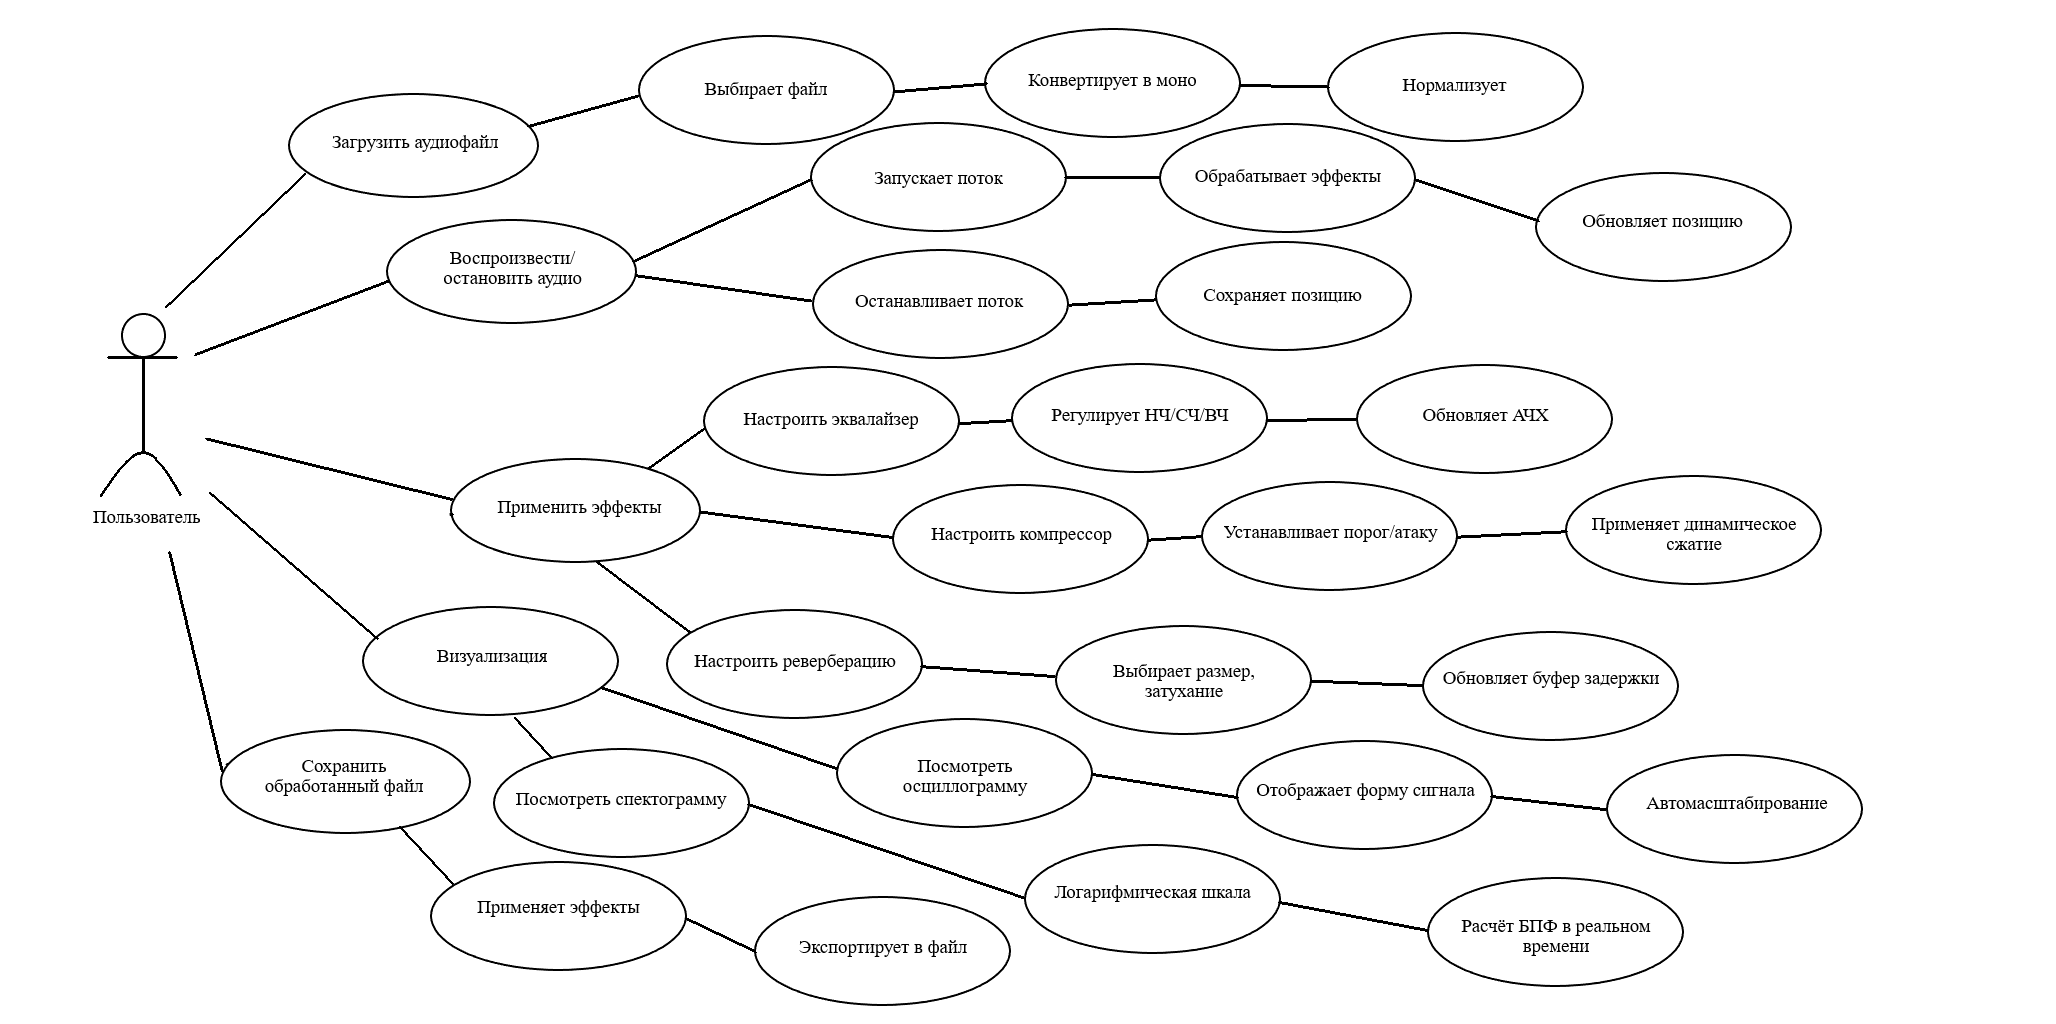
\includegraphics[width=1\linewidth]{DiagramPrec}}
	\caption{Диаграмма прецедентов}
	\label{fig:use_case_diagram}
\end{figure}

\paragraph{Вариант использования «Оформление заказа»}
Заинтересованные лица и их требования: пользователь хочет загрузить аудиофайл для последующей обработки.

Требования: поддержка форматов (WAV, MP3, OGG, FLAC), автоматическая конвертация в моно, нормализация амплитуды.

Предусловие: приложение запущено, файл существует и доступен для чтения.

Постусловие: аудиоданные загружены в память, форма волны отображена на графике, кнопки "Воспроизвести" и "Сохранить" активированы.

Основной успешный сценарий:
\begin{enumerate}
	\item Пользователь нажимает кнопку "Загрузить".
	\item Открывается диалоговое окно выбора файла.
	\item Пользователь выбирает файл и подтверждает выбор.
\end{enumerate}

\paragraph{Вариант использования «Воспроизведение аудио»}

Заинтересованные лица и их требования: пользователь хочет прослушать загруженный файл с возможностью применения эффектов в реальном времени.

Предусловие: аудиофайл успешно загружен, аудиоустройство вывода доступно.

Постусловие: аудиопоток запущен, графики обновляются в реальном времени.

Основной успешный сценарий:
\begin{enumerate}
	\item Пользователь нажимает кнопку «Воспроизвести».
	\item Система инициализирует аудиопоток
	\item Callback-функция начинает передавать данные в устройство.
	\item Позиция воспроизведения обновляется каждые 100 мс.
	\item Сигнал и АЧХ отображаются в реальном времени.
\end{enumerate}

\paragraph{Вариант использования «Остановка воспроизведения»}

Заинтересованные лица и их требования: пользователь хочет немедленно прекратить воспроизведение аудио.

Предусловие: идёт воспроизведение аудиофайла.

Постусловие: аудиопоток полностью остановлен, интерфейс обновлен.

Основной успешный сценарий:
\begin{enumerate}
	\item Пользователь нажимает кнопку "Стоп".
	\item Система останавливает воспроизведение аудио.
	\item Текущая позиция фиксируется для возможности дальнейшего продолжения.
\end{enumerate}

\paragraph{Вариант использования «Изменения позиции воспроизведения»}

Заинтересованные лица и их требования: пользователь хочет перемотать аудио на произвольную позицию.

Предусловие: аудиофайл загружен.

Постусловие: текущая позиция воспроизведения изменена, при активном воспроизведении звук продолжается с новой позиции, интерфейс синхронизирован.

Основной успешный сценарий:
\begin{enumerate}
	\item Пользователь перемещает ползунок позиции мышью.
	\item Система пересчитывает позицию.
	\item При воспроизведении поток начинает чтение с новой позиции.
\end{enumerate}

\paragraph{Вариант использования «Применения эквалайзера»}

Заинтересованные лица и их требования: пользователь хочет настроить частотный баланс (НЧ/СЧ/ВЧ).

Предусловие: файл загружен, вкладка "Эквалайзер" открыта.

Постусловие: параметры эквалайзера применены к аудиопотоку, график АЧХ обновлен.

Основной успешный сценарий:
\begin{enumerate}
	\item Пользователь включает чекбокс «Эквалайзер».
	\item Регулирует ползунки НЧ/СЧ/ВЧ.
	\item Система пересчитывает коэффициент БИХ-фильтров.
	\item Аудиозапись изменяется в соответствии с настройками пользователя.
	\item АЧХ отображается на графике.
\end{enumerate}

\paragraph{Вариант использования «Применения компрессора»}

Заинтересованные лица и их требования: пользователь хочет изменить динамический диапазон аудиосигнала для более равномерного звучания.

Предусловие: аудиофайл успешно загружен, вкладка "Компрессор" открыта.

Постусловие: параметры компрессора применены к аудиопотоку, изменения слышны при воспроизведении.

Основной успешный сценарий:
\begin{enumerate}
	\item Пользователь активирует чекбокс «Компрессор».
	\item Устанавливает порог, коэффициент компрессии, время атаки и восстановления, усиление выходного сигнала.
	\item Аудио обрабатывается в режиме реального времени.
\end{enumerate}

\paragraph{Вариант использования «Применения реверберации»}

Заинтересованные лица и их требования: пользователь хочет добавить эффект реверберации к аудиосигналу.

Предусловие: аудиофайл успешно загружен, вкладка "Реверберация" открыта.

Постусловие: эффект реверберации применен к аудиопотоку, буфер реверберации инициализирован с новыми параметрами.

Основной успешный сценарий:
\begin{enumerate}
	\item Пользователь активирует чекбокс "Реверберация".
	\item Пользователь регулирует параметры: уровень эффекта, исходный звук, размер комнаты, затухание.
	\item Аудио обрабатывается в режиме реального времени.
\end{enumerate}	

\paragraph{Вариант использования «Сохранение обработанного файла»}

Заинтересованные лица и их требования: пользователь хочет экспортировать результат с примененными эффектами.

Предусловие: файл загружен, эффекты настроены.

Постусловие: файл сохранен на диск в выбранном формате.

Основной успешный сценарий:
\begin{enumerate}
	\item Пользователь нажимает "Сохранить".
	\item Открывается диалог выбора формата (WAV/MP3) и пути.
	\item Пользователь выбирает формат, путь и название файла.
	\item Система применяет выбранные эффекты, экспортирует файл.
	\item Файл успешно сохранён на диске.
\end{enumerate}		

\paragraph{Вариант использования «Визуализация данных»}

Заинтересованные лица и их требования: пользователь хочет видеть графическое представление аудиосигнала.

Предусловие: аудиофайл загружен и идет воспроизведение.

Постусловие: графики формы волны и АЧХ отображаются и обновляются в режиме реального времени.

Основной успешный сценарий:
\begin{enumerate}
	\item Пользователь нажимает «Воспроизвести».
	\item Система отображает графики формы волны и АЧХ.
\end{enumerate}	

%-------------------------------------------------------------------------------
\subsubsection{Требования пользователя к интерфейсу веб-приложения}

Приложение должно иметь следующие основные функции:
\begin{enumerate}
	\item Основные элементы управления - кнопки управления воспроизведением: "Загрузить", "Воспроизвести", "Стоп", "Сохранить". Ползунок позиции воспроизведения, точное позиционирование, индикатор текущей позиции в формате MM:SS / MM:SS.
	\item Визуализация аудио - два синхронизированных графика: верхний график формы волны и нижний график амплитудно-частотной характеристики. Подписи осей с единицами измерения (амплитуда, частота).
	\item Панель эффектов (вкладки):
	\begin{enumerate}
		\item Эквалайзер - Три ползунка с подписями: низкие частоты (150Hz): ±24 дБ, средние частоты (1kHz): ±24 дБ, высокие частоты (5kHz): ±24 дБ. Чекбокс активации эффекта.
		\item Компрессор - ползунки параметров: порог: -60..0 дБ, соотношение: 1..20, атака: 1..500 мс, восстановление: 10..2000 мс, усиление: 0..24 дБ. Чекбокс активации эффекта.
		\item Реверберация: ползунки параметров: уровень эффекта: 0..1, сухой сигнал: 0..1, размер помещения: 0.1..2.0, затухание: 0.1..0.9. Чекбокс активации эффекта.
	\end{enumerate}	
	\item Обратная связь и состояние: индикатор загрузки при обработке файлов. Всплывающие уведомления об ошибках: при неудачной загрузке файла, при проблемах с аудиоустройством, при ошибках сохранения. Изменение состояния кнопок: "Воспроизвести" активна только при загруженном файле, "Стоп" активна только во время воспроизведения, "Сохранить" активна только после загрузки файла.
	\item Производительность: задержка отклика интерфейса не более 100 мс, плавная анимация графиков без рывков, минимальное потребление ресурсов в фоновом режиме.
\end{enumerate}	

\subsubsection{Нефункциональные требования к программной системе}

\paragraph{Требования к надёжности}

В процессе работы аудио-процессора могут возникнуть следующие аварийные ситуации:
\begin{itemize}
	\item потеря доступа к аудиоустройству в связи с его отключением, изменением системных настроек звука или конфликтом с другим приложением;
	\item попытка загрузки повреждённого или неподдерживаемого аудиофайла с несовместимым форматом, битрейтом или частотой дискретизации;
	\item неожиданное прекращение работы из-за нехватки системных ресурсов при обработке объёмных файлов или одновременном применении нескольких ресурсоёмких эффектов;
	\item ошибки в работе эффектов обработки звука, приводящие к искажению аудиосигнала или сбоям в воспроизведении.
\end{itemize}

Приложение должно автоматически определять доступные аудиоустройства и переключаться между ними при потере соединения с текущим устройством. В случае невозможности восстановления подключения система должна сохранять возможность обработки звука без функции воспроизведения с уведомлением пользователя о возникшей проблеме.

Для работы с аудиофайлами приложение должно проверять их целостность и соответствие поддерживаемым форматам перед загрузкой, а также автоматически выполнять необходимые преобразования (нормализацию, конвертацию в моно, приведение к стандартной частоте дискретизации). При обнаружении критических ошибок в файле пользователь должен получить понятное сообщение о проблеме с указанием конкретной причины.

Для предотвращения аварийного завершения из-за нехватки ресурсов система должна контролировать использование оперативной памяти и процессорного времени, ограничивать размеры буферов обработки и корректно завершать работу при приближении к предельным значениям. Все параметры эффектов и текущее состояние обработки должны сохраняться даже при аварийном завершении работы.

При возникновении ошибок в работе эффектов обработки звука система должна автоматически сбрасывать параметры эффектов к безопасным значениям, сохраняя при этом возможность дальнейшей работы. Все критические ошибки должны фиксироваться в системном логе с указанием времени возникновения, типа ошибки и состояния системы на момент сбоя.

\paragraph{Требования к безопасности}

Требования к приложению:
\begin{enumerate}
	\item Перед загрузкой файла, система должна проверять формат и корректность заголовков. При обнаружении повреждённых данных программа будет выводить ошибку без попытки обработки.
	\item Для безопасности управления памятью и ресурсами необходима изоляция обработки аудио, то есть каждый эффект будет применяться в отдельном потоке с контролем потребления ресурсов и будет ограничен буфе. Так же потребуется очистка временных данных, чтобы после завершения обработки или при ошибке все промежуточные буферы будут очищаться.
	\item Для защиты от вирусов применится проверка структуры файлов, анализ сигнатуры файла перед декодированием, ограничение максимальной длительности обрабатываемого аудио.
	\item Пользовательские настройки будут проверятся перед применением, а недопустимые значения автоматически скорректируются до ближайших безопасных.
	\item При завершении работы, приложение будет останавливать все потоки, освобождать аудиоустройства.
\end{enumerate}

\paragraph{Требования к программному обеспечению}

Для реализации программы будет использоваться язык программирования Python и библиотеки: NumPy, SciPy, PyDub, SoundDevice, Matplotlib, Numba.

Для работы приложения требуется Windows 10/11 (64-bit)

\paragraph{Требования к аппаратному обеспечению}

Минимальная конфигурация:

Центральный процессор с количеством ядер от 2 и выше с тактовой частотой от 2.0 ГГц. Поддержка инструкций SSE4.2. Оперативная память - 4 ГБ. 100 МБ свободного места для установки. Поддержка ASIO/WASAPI для профессионального использования.

\subsubsection{Требования к оформлению документации}

Требования к стадиям разработки программ и программной документации для вычислительных машин, комплексов и систем независимо от их назначения и области применения, этапам и содержанию работ устанавливаются ГОСТ 19.102-77
Программная документация должна включать в себя:
\begin{itemize}
	\item анализ предметной области;
	\item техническое задание;
	\item технический проект.
\end{itemize}

	\section{Технический проект}

\subsection{Общая характеристика организации решения задачи}

Необходимо спроектировать и разработать программный комплекс для обработки аудиосигналов, сочетающий функциональность профессиональных аудиоредакторов с простотй и удобством интерфейса.

В приложении должно быть:
\begin{itemize}
	\item модульная структура с чётким разделением на: ядро обработки, пользовательский интерфейс, системную обвязку;
	\item гибкая система эффектов: трёхполосный параметрический эквалайзер с настраиваемыми частотами среза, компрессор с регулируемыми параметрами, алгоритм реверберации;
	\item оптимизированная обработки сигнала: поддержка многопоточной обработки для работы в реальном времени, аппаратно-независимая реализация звукового движка, автоматическая нормализация входного и выходного сигнала;
	\item интерактивная визуализация; формы волны во временной области, АЧХ применяемых фильтров.
\end{itemize}
 
\subsection{Обоснование выбора технологий проектирования}

Используемые для создания программно-информационной системы языки и технологии отвечают современным практикам разработки, позволяют достичь высокой производительности и отказоустойчивости программы.

\subsubsection{Язык программирования Python}

Python - основной язык разработки проекта. Python выбран благодаря своей гибкости, богатой экосистеме библиотек и кроссплатформенной поддержке. Его синтаксис позволяет быстро разрабатывать сложные алгоритмы обработки сигналов, а динамическая типизация упрощает интеграцию с различными аудиоформатами и устройствами.

Используемые библиотеки:
\begin{itemize}
	\item NumPy - обеспечивает высокопроизводительные вычисления с многомерными массивами, что критично для обработки аудиоданных, представленных в виде временных рядов;
	\item SciPy - используется для реализации цифровых фильтров (эквалайзер), БПФ (анализ спектра) и других математических операций;
	\item PyDub - библиотека для работы с аудиофайлами, предоставляющая: простые методы загрузки и сохранения в форматах WAV, MP3, OGG, FLAC, базовые операции, такие как обрезка, наложение, изменение громкости, конвертация частоты дискретизации, интеграцию с FFmpeg для поддержки дополнительных кодеков;
	\item SoundDevice - обеспечивает низкоуровневый доступ к аудиоустройствам через PortAudio. Ключевые функции: воспроизведение и запись в реальном времени с минимальной задержкой, поддержка ASIO, WASAPI, Core Audio для профессиональных аудиоинтерфейсов, гибкая настройка параметров потока: частота дискретизации, размер буфера, количество каналов;
	\item Matplotlib - используется для визуализации аудиоданных: построение осциллограмм (форма сигнала во временной области), отображение АЧХ (амплитудно-частотных характеристик) с логарифмической шкалой, интерактивное обновление графиков в реальном времени;
	\item Tkinter - стандартная библиотека Python для создания графического интерфейса. В проекте применяется для: построения основного окна с вкладками (эквалайзер, компрессор, реверберация), реализации интерактивных элементов: ползунки, кнопки, метки, интеграции графиков Matplotlib через FigureCanvasTkAgg;
	\item Numba - JIT-компилятор для оптимизации вычислительно сложных участков кода: ускорение алгоритмов компрессии и реверберации в 5–10 раз, поддержка многопоточности.
\end{itemize}

\subsubsection{Кроссплатформенная библиотека FFmpeg}

FFmpeg — это мощная кроссплатформенная библиотека для обработки мультимедиа, используемая в проекте для работы с аудиофайлами различных форматов. Взаимодействие с FFmpeg осуществляется через обёртку PyDub, что значительно упрощает операции чтения, записи и конвертации аудио.

Основные функции FFmpeg в проекте:
\begin{enumerate}
	\item Поддержка множества аудиоформатов. Позволяет загружать и сохранять файлы в форматах: без сжатия: WAV, AIFF, с потерями: MP3, AAC, OGG, без потерь: FLAC, ALAC. Обеспечивает автоматическое определение кодека при загрузке.
	\item Конвертация аудио: изменение частоты дискретизации, преобразование между форматами, конвертация числа каналов.
	\item Нормализация и обработка. Автоматическая регулировка громкости.
\end{enumerate}

FFmpeg был выбран по рядам преимуществ:
\begin{itemize}
	\item универсальность: поддержка 100+ кодеков и контейнеров;
	\item стабильность: отлаженные алгоритмы декодирования/кодирования;
	\item производительность: оптимизированные нативные библиотеки;
	\item гибкость: Возможность тонкой настройки параметров через командные опции.
\end{itemize}

\subsection{Архитектура программной системы}

На рисунке \ref{DiagramArch:image} представлена многослойная архитектура системы с чётким разделение ответственности между компонентами.

\begin{figure}[p]  % Разместить на отдельной странице
	\centering
	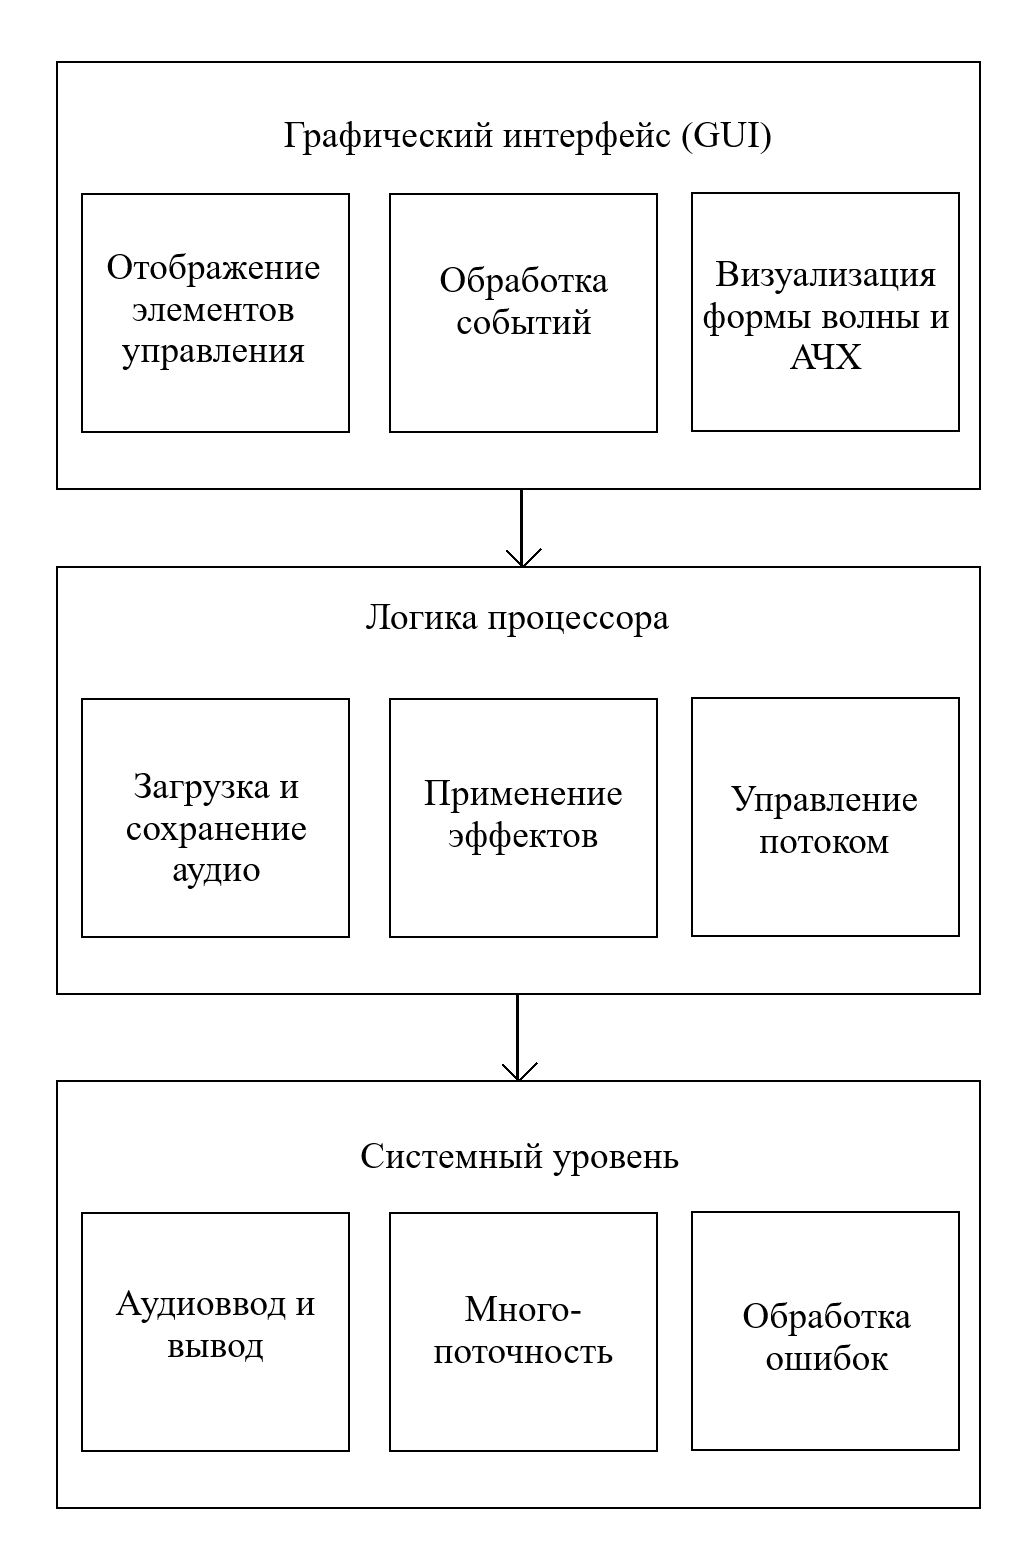
\includegraphics[width=0.8\linewidth]{DiagramArch}
	\caption{Архитектура программной системы}
	\label{DiagramArch:image}
\end{figure}
\clearpage

\begin{enumerate}
	\item Графический интерфейс отображает элементы управления (кнопки, ползунки, вкладки), визуализирует аудиоданные в реальном времени (Осциллограмма, АЧХ), обрабатывает пользовательские события (нажатия кнопок, изменение параметров).
	\item Логика процессора отвечает за загрузку/сохранение аудио, чтение файлов через PyDub/FFmpeg, конвертирует в формат float32 для обработки. Применяет эффекты: эквалайзер (БИХ-фильтры для НЧ/СЧ/ВЧ), компрессор (динамическое сжатие с параметрами), реверберация. Буферизирует данные и синхронизирует позицию воспроизведения.
	\item На уровне системы происходит ввод и вывод аудио, создаётся отдельный поток для обработки аудио и очереди для передачи данных между потоками. Обрабатываются ошибки, перехватываются исключения и логируются в файл.
\end{enumerate}

\subsection{Компоненты программы}

Приложение Audio Processor состоит из следующих ключевых компонентов, организованных в модульную структуру:
\begin{itemize}
	\item графический интерфейс включает главное окно, состоящее из кнопок управление воспроизведением и загрузки/сохранения, вкладок эффектов (эквалайзер, компрессор и ревербератор), окна отображение визуализации формы волны и АЧХ;
	\item логика процессора читает и обрабатывает аудиофайлы, применяется выбранные эффекты по очереди, управляет всей работой программы;
	\item системное устройство воспроизводит звук, работает с файлами, открывает и сохраняет их, управляет несколькими задачами одновременно;
	\item вспомогательные модули включают частотный анализ, автоматически регулирует громкость и записывает ошибки и события.
\end{itemize}

Все части программы взаимодействуют между собой по чётким правилам. Когда пользователь меняет настройки, интерфейс передаёт их в модуль обработки, который применяет эффекты и отправляет результат на воспроизведение и отображение. Для плавной работы использовались очереди задач для работы в многопоточном режиме, оптимизирует сложные вычисления для быстрой работы.

\subsection{Архитектура приложения}
Приложение построено по многослойной модульной архитектуре с разделением на логические компоненты, взаимодействующие через четко определенные интерфейсы. В основе лежит ядро обработки аудиосигналов, окруженное графическим интерфейсом, системными сервисами и вспомогательными модулями.
Графический интерфейс реализован на Tkinter и включает:
\begin{itemize}
	\item главное окно (MainWindow) с вкладками для управления эффектами, кнопками воспроизведения/паузы и областью визуализации;
	\item панель эквалайзера (EQPanel) с тремя ползунками (НЧ/СЧ/ВЧ), отображающая АЧХ через Matplotlib;
	\item панель компрессора (CompressorPanel) для настройки порога, сжатия, атаки, восстановления, усиления;
	\item панель реверберации (ReverbPanel) для настройки эффект, сухой сигнал, размер комнаты, затухание;
	\item визуализатор спектра (SpectrumAnalyzer), отображающий осциллограмму (форма сигнала) и частотный спектр (БПФ) в реальном времени;
	\item прогресс-бар с управлением позицией воспроизведения и отображением длительности трека.	
\end{itemize}

Логический процессор — центральный модуль, отвечающий за:
\begin{itemize}
	\item загрузку и конвертацию аудио через PyDub (с использованием FFmpeg как бэкенда), включая поддержку WAV, MP3, FLAC;
	\item эквалайзер на БИХ-фильтрах с частотами 150 Гц (НЧ), 1 кГц (СЧ), 5 кГц (ВЧ);
	\item компрессор с параметрами knee, makeup gain;
	\item реверберация на основе алгоритма Schroeder (комбинация линий задержки и FIR-фильтров);
	\item буферизацию данных для плавного воспроизведения и нормализацию уровня сигнала.
\end{itemize}

Системный слой обеспечивает интеграцию с ОС и оборудованием:
\begin{itemize}
	\item аудиопоток (AudioStream) на базе SoundDevice, обрабатывающий ввод/вывод в реальном времени с настройкой latency и sample rate (44.1–192 кГц);
	\item менеджер потоков (ThreadManager) для параллельной обработки (отдельные потоки для: GUI, аудиообработки, визуализации);
	\item файловый менеджер (FileManager) с кэшированием загруженных треков и поддержкой метаданных (ID3-теги).
\end{itemize}

Архитектура обеспечивает масштабируемость (добавление новых эффектов через модули), производительность (JIT-компиляция, многопоточность) и отказоустойчивость (изоляция сбоев в отдельных потоках).

\subsection{Проект данных программной системы}

Система оперирует тремя основными категориями данных: входными, промежуточными и выходными. Входные данные включают аудиофайлы в форматах WAV, MP3, FLAC и OGG с поддержкой различных характеристик (битность 16-24 бит, частота дискретизации 44.1-192 кГц), а также параметры эффектов, настраиваемые пользователем через графический интерфейс. Для эквалайзера это уровни усиления по трём полосам (низкие на 150 Гц, средние на 1 кГц, высокие на 5 кГц с диапазоном ±24 дБ), для компрессора — порог срабатывания от -60 до 0 дБ, коэффициент компрессии от 1:1 до 20:1, время атаки и восстановления от 0.1 до 500 мс, для реверберации — соотношение обработанного и исходного сигнала, коэффициент затухания и виртуальный размер помещения.

Промежуточные данные представлены в виде нормализованных аудиобуферов в формате 32-битных чисел с плавающей запятой, организованных как моно- или стереоканальные массивы. Система использует кольцевые буферы для обработки в реальном времени и промежуточные спектральные данные, полученные через быстрое преобразование Фурье с применением оконной функции. Для хранения состояния эффектов используются специализированные структуры: коэффициенты БИХ-фильтров эквалайзера, параметры огибающей компрессора и линии задержки реверберации.

Выходные данные включают обработанные аудиофайлы в выбранных пользователем форматах (WAV с PCM-кодированием или MP3 с переменным битрейтом), сохраняющие исходные параметры частоты дискретизации или конвертируемые к стандартным значениям. Визуализационные данные содержат три основных компонента: осциллограмму последних обработанных сэмплов, частотный спектр с разрешением 8192 точек и амплитудно-частотную характеристику активных фильтров, отображаемую в логарифмическом масштабе от 20 Гц до 20 кГц.

Метаданные системы включают пользовательские пресеты эффектов, содержащие полный набор параметров обработки, историю операций для возможности отмены действий, а также технические лог-файлы с информацией о производительности и ошибках. Все данные передаются между компонентами системы через единый формат аудиоблоков, сопровождаемых метаинформацией о текущих настройках обработки, что обеспечивает согласованность работы многопоточной архитектуры.

\subsubsection{Описание сущностей графического интерфейса}

Графический интерфейс Audio Processor представляет собой комплекс взаимосвязанных визуальных компонентов, объединенных в единое интуитивное пространство. 

Интерфейс поддерживает несколько режимов отображения - компактный для мониторов с малым разрешением, расширенный с дополнительными инструментами анализа для профессиональной работы, и режим презентации с увеличенными элементами управления. Все визуальные компоненты реализованы с учетом эргономики - важные элементы выделены акцентным цветом, соблюдены принципы визуальной иерархии, обеспечена последовательная реакция на пользовательские действия. Особенностью интерфейса является синхронизация всех элементов - изменения параметров эффектов мгновенно отражаются на графиках, а действия пользователя сопровождаются тактильной обратной связью в виде тонких анимационных эффектов.

\subsubsection{Описание сущностей логики процессора}

Основу обработки составляет низкоуровневый модуль, работающий с потоком аудиосэмплов в формате 32-битных чисел с плавающей точкой, обеспечивающий базовые операции нормализации и передискретизации. Система эффектов построена вокруг трех ключевых процессоров: эквалайзер реализует трехполосную фильтрацию через каскад БИХ-фильтров с настраиваемыми частотами среза и коэффициентами усиления, компрессор отвечает за компрессию сигнала с алгоритмами расчета огибающей и адаптивными параметрами атаки/восстановления, а ревербератор генерирует реверберацию через комбинацию линий задержки с регулируемыми параметрами затухания.

Поток данных управляется специализированным менеджером маршрутизации, который обеспечивает передачу аудиоблоков между модулями с минимальной задержкой, используя кольцевые буферы и механизм синхронизации для многопоточной работы. Состояние системы отслеживает активные эффекты, параметры обработки и текущий режим работы (реальное время/оффлайн обработка), предоставляя единый интерфейс для управления конвейером обработки. 

\subsubsection{Описание сущностей системного уровня}

Системная архитектура приложения построена на нескольких ключевых компонентах, обеспечивающих интеграцию с операционной средой и аппаратными ресурсами. Центральным элементом выступает абстрактный слой взаимодействия с аудиодрайверами, реализующий поддержку ASIO, WASAPI и Core Audio через единый кроссплатформенный API. Для управления устройствами ввода-вывода используется DeviceManager, который автоматически обнаруживает доступные аудиоинтерфейсы, анализирует их характеристики и предоставляет унифицированный интерфейс для работы с ними.

Файловая подсистема основана на компоненте, объединяющем возможности стандартных Python-библиотек для работы с файлами и мощь FFmpeg для обработки мультимедиа. Этот модуль включает кэширующий механизм для ускорения повторного доступа к аудиофайлам и систему контроля целостности данных. 

Многопоточная архитектура координируется центральным диспетчером задач, который создает и управляет тремя основными типами потоков: высокоприоритетным аудиопотоком реального времени, фоновыми рабочими потоками для обработки эффектов и служебными потоками для визуализации и логирования.

\subsection{Проектирования пользовательского интерфейса}

Центральное место занимает динамическая визуализация аудиопотока - двойной дисплей с синхронизированными осциллограммой и АЧХ, выполненный в темной цветовой гамме с акцентными элементами салатового цвета для выделения ключевых параметров сигнала. Основная рабочая область: верхняя треть экрана отведена под графики, центральная часть содержит компактные панели эффектов с интуитивными регуляторами, а нижний сектор занимает расширенная панель транспорта с профессиональными элементами управления.

Навигационная система реализована через адаптивную панель вкладок с контекстно-зависимыми элементами управления - при выборе конкретного эффекта (эквалайзер, компрессор, реверберация) нижняя панель автоматически наполняется соответствующими регуляторами, сохраняя при этом быстрый доступ к основным функциям. Все элементы управления спроектированы с учетом тактильного взаимодействия - ползунки имеют выраженные рифленые ручки с магнитными точками для часто используемых значений, кнопки обладают трехступенчатой визуальной обратной связью (покой, наведение, нажатие), а переключатели сопровождаются мягкими анимационными переходами.

На рисунке 3.2 представлен интерфейс программы при запуске. Макет содержит следующие элементы:
\begin{enumerate}
	\item Окно вывода графика формы волны.
	\item Окно вывода АЧХ.
	\item Активная кнопка для загрузки аудио.
	\item Активная кнопка для воспроизведения аудио.
	\item Не активная кнопка для остановки аудио.
	\item Не активная кнопка для сохранения аудио.
	\item Вкладка выбора эффекта эквалайзер (выбран).
	\item Вкладка выбора эффекта компрессор (не выбран).
	\item Вкладка выбора эффекта реверберации (не выбран).
	\item Бегунок регулировки низких частот.
	\item Бегунок регулировки средних частот.
	\item Бегунок регулировки высоких частот.
	\item Чекбокс включения эквалайзера.
	\item Бегунок управления временем начала воспроизведения.
	\item Время, в которое воспроизводится аудио и полная длина файла.
\end{enumerate}

\begin{figure}[ht]
	\center{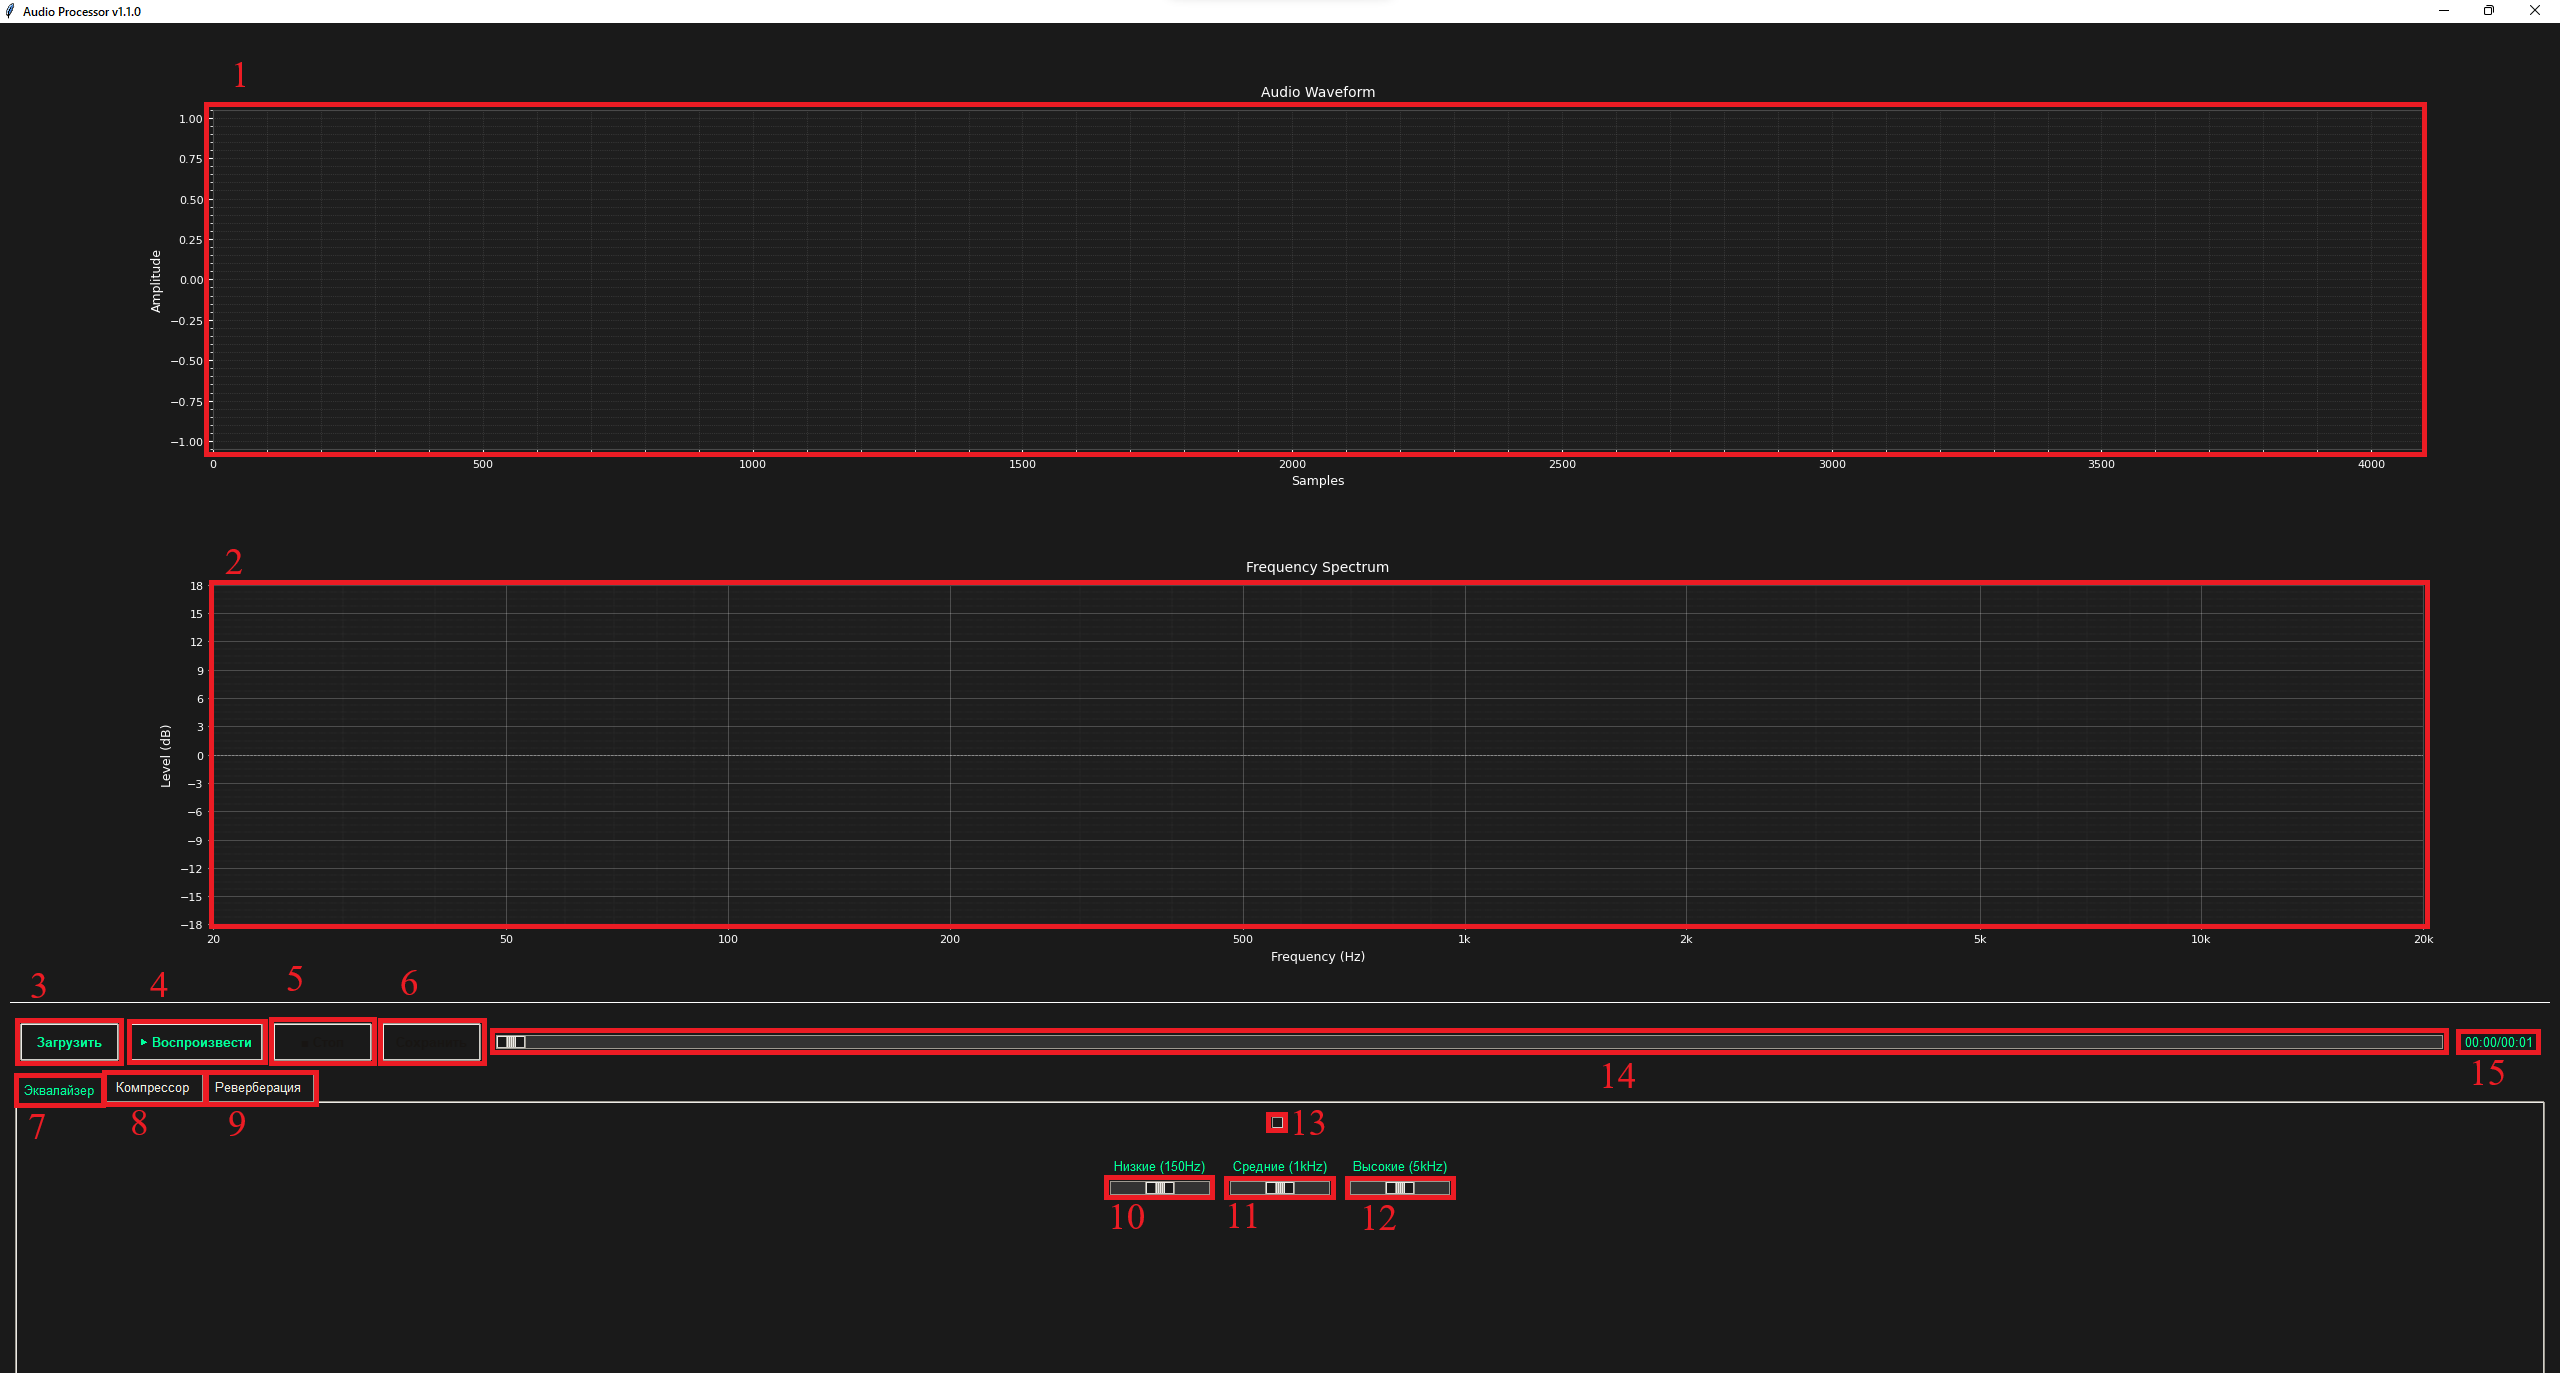
\includegraphics[width=0.8\linewidth]{1}}
	\caption{Макет интерфейса программы}
	\label{1:image}
\end{figure}
\clearpage

На рисунке 3.3 изображён макет вкладки компрессора. Макет содержит следующие элементы:
\begin{enumerate}
	\item Бегунок настройки порогового значения.
	\item Бегунок настройки параметров сжатия.
	\item Бегунок настройки времени атаки в миллисекундах.
	\item Бегунок настройки времени восстановления сигнала в миллисекундах.
	\item Бегунок настройки усиления выходного сигнала.
	\item Чекбокс включения эффека.
\end{enumerate}

\begin{figure}[ht]
	\center{
\includegraphics[width=1\linewidth]{2}}
	\caption{Макет окна компрессора}
	\label{2:image}
\end{figure}

На рисунке 3.4 изображён макет вкладки реверберации. Макет содержит следующие элементы:
\begin{enumerate}
	\item Бегунок настройки уровня эффекта.
	\item Бегунок настройки исходного звука.
	\item Бегунок настройки размера пространства.
	\item Бегунок настройки затухания.
	\item Чекбокс включения эффекта.
\end{enumerate}

\begin{figure}[ht]
	\center{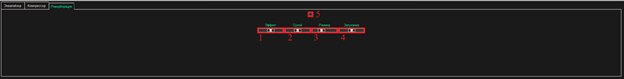
\includegraphics[width=1\linewidth]{3}}
	\caption{Макет окна реверберации}
	\label{3:image}
\end{figure}
\clearpage
	\ifПрактика{}\else{
		\section{Рабочий проект}
\subsection{Классы, используемые при разработке сайта}

Можно выделить следующий список классов и их методов, использованных при разработке веб-приложения (таблица \ref{class:table}).

\renewcommand{\arraystretch}{0.8} % уменьшение расстояний до сетки таблицы
\begin{xltabular}{\textwidth}{|X|p{2.5cm}|>{\setlength{\baselineskip}{0.7\baselineskip}}p{4.85cm}|>{\setlength{\baselineskip}{0.7\baselineskip}}p{4.85cm}|}
\caption{Описание классов, используемых в приложении\label{class:table}}\\
\hline \centrow \setlength{\baselineskip}{0.7\baselineskip} Название класса & \centrow \setlength{\baselineskip}{0.7\baselineskip} Модуль, к которому относится класс & \centrow Описание класса & \centrow Методы \\
\hline \centrow 1 & \centrow 2 & \centrow 3 & \centrow 4\\ \hline
\endfirsthead
\caption*{Продолжение таблицы \ref{class:table}}\\
\hline \centrow 1 & \centrow 2 & \centrow 3 & \centrow 4\\ \hline
\finishhead
Validator & Валидатор & Validator - реализует логику валидации и проверки данных, которые намереваются отправить в sql, для поддержания её стабильности & required - проверка наличия значения, type - numeric, date, string, max - ограничение длины строки, pattern - валидация email/телефона, foreign - cуществование в связанной таблице.\\
\hline * & * & * & *
\end{xltabular}
\renewcommand{\arraystretch}{1.0} % восстановление сетки

\newpage 
\subsection{Описание элементов интерфейса пользователя}

На рисунке \ref{index:image} главная страница сайта Pc-Club содержит информацию, навигацию, пример работ.

\begin{enumerate}
	\item Панель навигации.
	\item Переход на страницу админ панели.
	\item Переход на страницу оформления.
	\item Смена учетной записи.
	\item Информационный блок.
	\item Переход к оформлению.
	\item Информационный блок, преимущества Pc-Club.
	\item Блок с примерами работ.
	\item Кастомный скролл.
	\item footer сайта с информацией.
\end{enumerate}

\begin{figure}[ht]
\center{\includegraphics[width=1\linewidth]{index}}
\caption{Главная страница сайта.}
\label{index:image}
\end{figure}

\newpage 
На рисунке \ref{main:image} представлено меню оформления заказа,  в каждом поле можно вписать вручную или выбрать из выпадающего списка.
\begin{enumerate}
	\item Переход на страницу админ панели.
	\item Переход на главную страницу.
	\item Смена учетной записи.
	\item Простая форма ввода только чисел для цены.
	\item Форма ввода с календарем для вывода дат, проверяет на корректность.
	\item Простая форма ввода для адреса.
	\item Выбор из выпадающего списка.
	\item Выбор из выпадающего списка с возможностью ручного ввода.
	\item Кнопка собирает информацию с форм и отправляет в sql.
	\item Выпадающее меню.
	\item Поле ручного ввода/поиска по компонентам в sql.
	\item Кнопка развернуть.
	\item Виды комплектующих из sql.
	\item Сколько этих комплектующих осталось на складе.
\end{enumerate}

\begin{figure}[H]
\center{\includegraphics[width=0.9\linewidth]{order+fl}}
\center{\includegraphics[width=0.9\linewidth]{order+fln}}
\center{\includegraphics[width=0.75\linewidth]{chosenone}}
\caption{Страница оформления заказа и выпадающее меню компонента.}
\label{main:image}
\end{figure}

На рисунке \ref{login:image} меню для авторизации пользователей в системе, после авторизации под админской учетной записью можно получить доступ к админ панели, складу.
\begin{enumerate}
	\item Форма ввода логина.
	\item Форма ввода пароля.
	\item Кнопка сравнивает логин и хэш пароля с хранящимся в sql, при совпадении пропускает.
	\item Кнопка сохраняет логин и хэш пароля в sql.
	\item Вернуться на главную страницу.
\end{enumerate}
\begin{figure}[ht]
	\center{\includegraphics[width=0.25\linewidth]{login}}
	\caption{Разделы для каждого вида компонентов.}
	\label{login:image}
\end{figure}

На рисунке \ref{adminall:image} Панель администратора Pc-Club позволяет полностью контролировать и редактировать информацию в sql.

\begin{enumerate}
	\item Панель навигации по сайту.
	\item Открыть меню выбора компонента.
	\item Ручной поиск по позициям и кнопка.
	\item Добавление новой записи в sql, через админ панель можно напрямую добавить новые компоненты в sql для их дальнейшего использования.
	\item Кнопка для редактирования, можно редактировать любую запись сделаную в таблицы sql.
	\item Кнопка для удаления, удалить любую запись из sql.
	\item Заголовок таблицы, в нашем случае для заказов.
	\item Контент таблицы, хранимый и извлеченный из sql.
\end{enumerate}

\begin{figure}[ht]
\center{\includegraphics[width=1\linewidth]{adminall}}
\caption{Админ-панель Pc-Club общий вид}
\label{adminall:image}
\end{figure}

На рисунке \ref{razdeli:image} меню выбора между типом компонентов в панели админа.

\begin{figure}[htbp]
\center{\includegraphics[width=0.25\linewidth]{razdeli}}
\caption{Разделы для каждого вида компонентов.}
\label{razdeli:image}
\end{figure}

На рисунке \ref{storedf:image} меню менеджмента склада для веб-приложения, здесь можно пополнять запасы недостающих комплектующих, потом применять их в заказах.

\begin{enumerate}
	\item Расширенная навигационная панель админа.
	\item Кнопка вызова меню выбора типа компонента.
	\item Ручной поиск по позициям и кнопка.
	\item Заголовок таблицы.
	\item Компонент из таблицы.
	\item Количество компонента на складе и поле для ввода нового значения.
	\item Кнопка для обновления значения.
\end{enumerate}

\begin{figure}[ht]
	\center{\includegraphics[width=1\linewidth]{storedf}}
	\caption{Страничка склада корпусов в качестве примера.}
	\label{storedf:image}
\end{figure}
\clearpage

		\section*{ЗАКЛЮЧЕНИЕ}
\addcontentsline{toc}{section}{ЗАКЛЮЧЕНИЕ}

И так в чем же преимущества веб-приложения? Главенствующим преимуществом системы для сервис центра является удобство и оперативность связи с клиентами, автоматизация части ручных процессов. При наличии всех вышеназванных плюсов стоит учитывать спецификацию бизнеса и целесообразность разработки.
  
Компании стремятся привлечь новых клиентов и автоматизировать часть ручной работы, ускорить некоторые процессы и увеличить прибыль. Для Pc-Club было разработано веб-приложение упрощающее работу сервис центра, а также привлекающее новых потенциальных клиентов.

Основные результаты работы:

\begin{enumerate}
\item Проведен анализ предметной области.
\item Разработана концептуальная модель веб-приложение. Разработана модель данных системы. Определены требования к системе. Разработана схема базы данных.
\item Осуществлено проектирование веб-приложение. Разработан пользовательский интерфейс приложения.
\item Реализован и протестирован веб-приложение. Проведено модульное и системное тестирование.
\end{enumerate}

Все требования, объявленные в техническом задании, были полностью реализованы, все задачи, поставленные в начале разработки проекта, были также решены.

Готовый рабочий проект представляет собой базу данных sql и веб-приложение.
	}\fi
	\addcontentsline{toc}{section}{СПИСОК ИСПОЛЬЗОВАННЫХ ИСТОЧНИКОВ}

\begin{thebibliography}{9}

    \bibitem{bib1} 
    Стоян Стефанов, JavaScript. Шаблоны / Стоян Стефанов – Москва: Символ-Плюс, 2011. – 262 с. – ISBN 978-5-93286-208-7 – Текст : непосредственный.
    
     \bibitem{bib2} 
    Васильев, В. И. Информационные системы / В. И. Васильев. – Москва: Финансы и статистика, 2009. – 416 с. – ISBN 978-5-279-03153-4. – Текст : непосредственный.
    
    \bibitem{bib3} 
    Гамзатов, М. Г. Информационные технологии / М. Г. Гамзатов, И. Г. Ахмедов. – Москва: Юрайт, 2018. – 392 с. – ISBN 978-5-534-05640-2. – Текст : непосредственный.
    
    \bibitem{bib4} 
    Голицына, О. Л. Информационные системы / О. Л. Голицына, Н. В. Максимов, И. И. Попов. – Москва: Форум, 2008. – 496 с. – ISBN 978-5-91134-245-4. – Текст : непосредственный.
    
    \bibitem{bib5} 
    Дейт, К. Введение в системы баз данных / К. Дейт. – Москва: Вильямс, 2006. – 1328 с. – ISBN 5-8459-0788-8. – Текст : непосредственный.
    
    \bibitem{bib6} 
    Информационные технологии: учебник для вузов / под ред. Н. В. Макаровой. – Москва: Финансы и статистика, 2005. – 768 с. – ISBN 5-279-02207-8. – Текст : непосредственный.
    
    \bibitem{bib7} 
    Кнут, Д. Искусство программирования / Д. Кнут. – Москва: Вильямс, 2000. – Т. 1. – 720 с. – ISBN 5-8459-0080-8. – Текст : непосредственный.
    
    \bibitem{bib8} 
    Кузнецов, С. В. Базы данных: учебник / С. В. Кузнецов. – Москва: Академия, 2007. – 496 с. – ISBN 978-5-7695-2477-0. – Текст : непосредственный.
    
    \bibitem{bib9}
    Литвиненко, В. В. Разработка информационных систем / В. В. Литвиненко. – Москва: Юрайт, 2018. – 344 с. – ISBN 978-5-534-07421-5. – Текст : непосредственный.
    
    \bibitem{bib10}
    Маклаков, С. В. BPWin и ERWin. CASE-средства разработки информационных систем / С. В. Маклаков. – Москва: ДИАЛОГ-МИФИ, 2000. – 304 с. – ISBN 5-86404-090-3. – Текст : непосредственный.
    
    \bibitem{bib11}
    Титтел, Э. HTML5 и CSS3 для чайников / Э. Титтел, К. Минник. – Москва: Вильямс, 2016. – 400 с. – ISBN 978-1-118-65720-1. – Текст : непосредственный.
    
    \bibitem{bib12}
    Новиков, Ф. А. Дискретная математика для программистов / Ф. А. Новиков. – Санкт-Петербург: Питер, 2000. – 304 с. – ISBN 5-272-00176-4. – Текст : непосредственный.
    
    \bibitem{bib13}
    Робертсон, С. Осваиваем SQL за 24 часа / С. Робертсон. – Москва: Вильямс, 2002. – 272 с. – ISBN 5-8459-0315-7. – Текст : непосредственный.
    
    \bibitem{bib14}
    Таненбаум, Э. Современные операционные системы / Э. Таненбаум. – Санкт-Петербург: Питер, 2002. – 1040 с. – ISBN 5-318-00299-4. – Текст : непосредственный.
    
    \bibitem{bib15}
    Мартин, Д. Организация баз данных в вычислительных системах / Д. Мартин. – Москва: Мир, 1980. – 662 с. – Текст : непосредственный.

    
    \bibitem{bib16}
    Электронный ресурс]. – URL: http://www.website.com (дата обращения: 15.05.2023). – Текст : электронный.
    
    \bibitem{bib17}
    Иванов, И. И. Анализ предметной области [Электронный ресурс] / И. И. Иванов. – Режим доступа: URL: http://www.example.com/ivanov (дата обращения: 20.05.2023). – Текст : электронный.
    
    \bibitem{bib18}
    Петров, П. П. Разработка информационной системы [Электронный ресурс] / П. П. Петров. – Режим доступа: URL: http://www.example.com/petrov (дата обращения: 25.05.2023). – Текст : электронный.
    
    \bibitem{bib19}
    Сидоров, С. С. Тестирование программного обеспечения [Электронный ресурс] / С. С. Сидоров. – Режим доступа: URL: http://www.example.com/sidorov (дата обращения: 30.05.2023). – Текст : электронный.
    
    \bibitem{bib20}
    Смирнов, А. А. Введение в базы данных [Электронный ресурс] / А. А. Смирнов. – Режим доступа: URL: http://www.example.com/smirnov (дата обращения: 05.06.2023). – Текст : электронный.
\end{thebibliography}

	\ifВКР{\appendix{Представление графического материала}

Графический материал, выполненный на отдельных листах,
изображен на рисунках А.1--А.\arabic{числоПлакатов}.
\setcounter{числоПлакатов}{0}

\renewcommand{\thefigure}{А.\arabic{figure}} % шаблон номера для плакатов

\begin{landscape}

\begin{плакат}
    
\includegraphics[width=0.82\linewidth]{плакат1.png}
    \заголовок{Сведения о ВКРБ}
    \label{pl1:image}      
\end{плакат}

\begin{плакат}
    
\includegraphics[width=0.82\linewidth]{плакат2.png}
    \заголовок{Цель и задачи разработки}
    \label{pl2:image}      
\end{плакат}

\begin{плакат}
    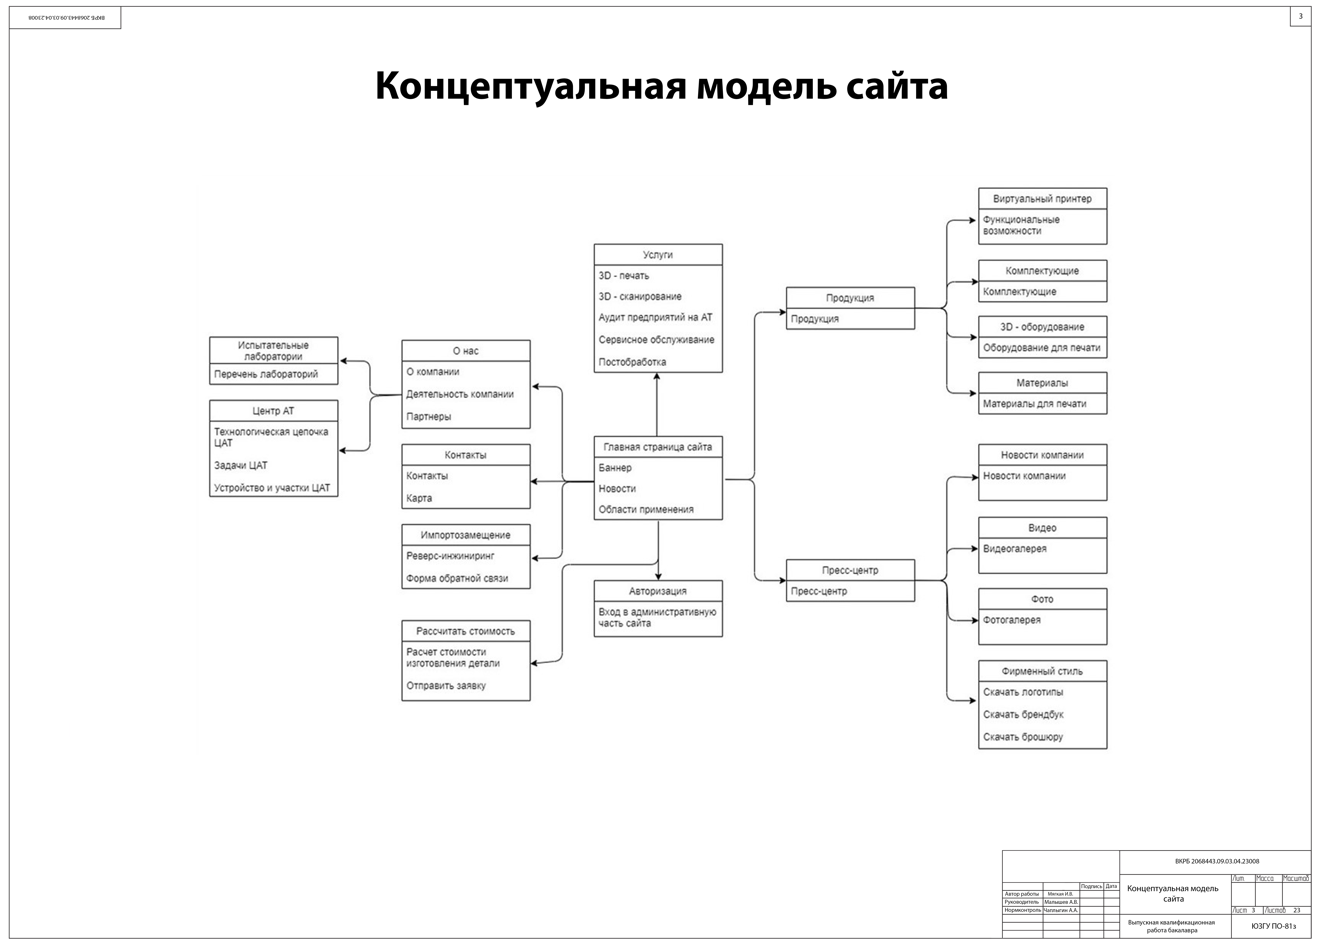
\includegraphics[width=0.82\linewidth]{плакат3.png}
    \заголовок{Концептуальная модель сайта}
    \label{pl3:image}      
\end{плакат}

\begin{плакат}
    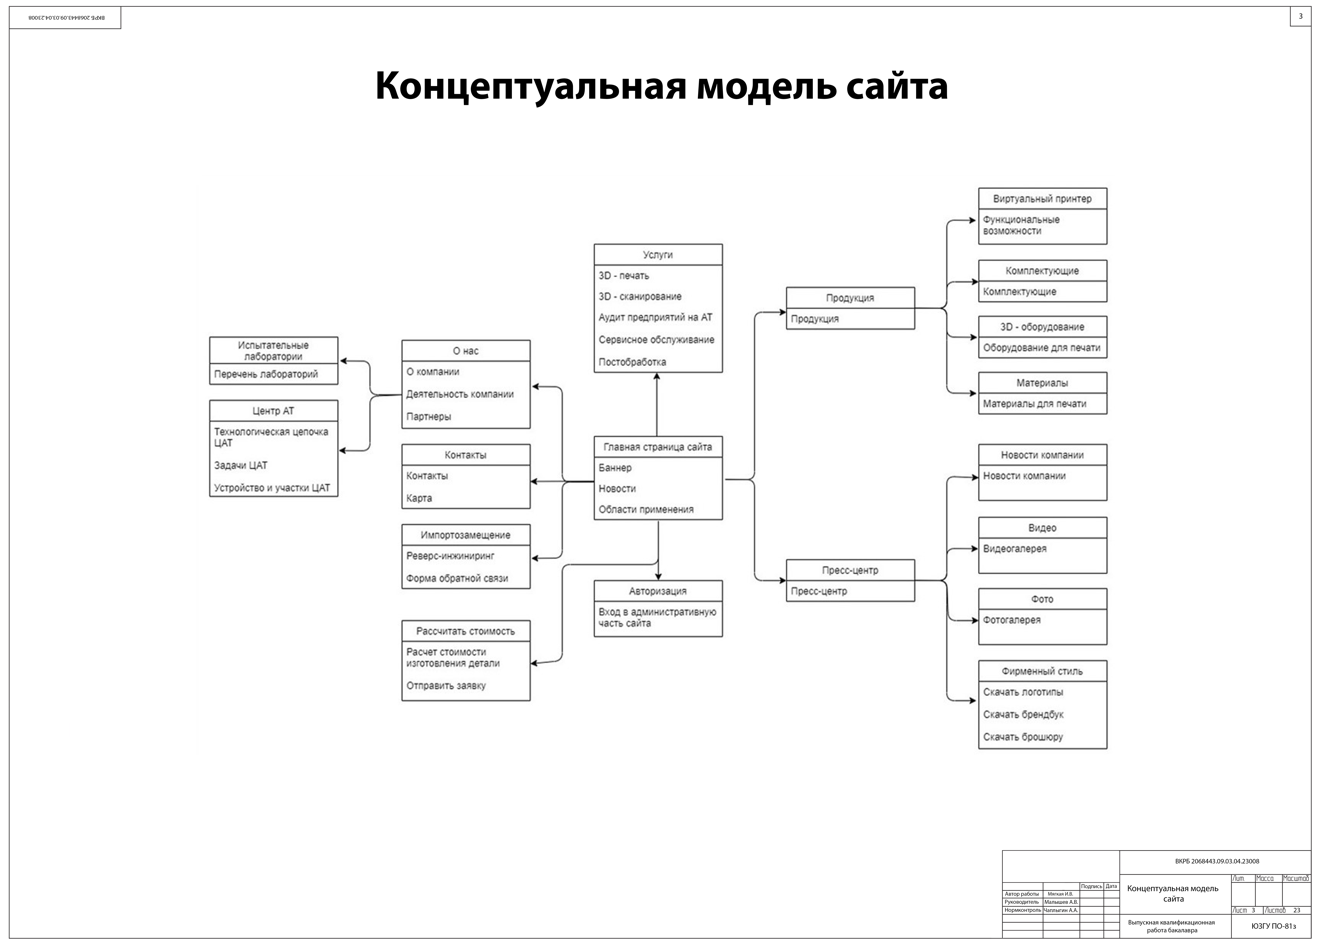
\includegraphics[width=0.82\linewidth]{плакат3.png}
    \заголовок{Еще плакат}
    \label{pl4:image}      
\end{плакат}

\end{landscape}
}\fi
	\ifПрактика{}\else{\appendix{Фрагменты исходного кода программы}


Orderform.php
\begin{figure}[ht]
	\begin{lstlisting}[language=Php]
		// Функция получения компонентов и загрузка данных
		function getComponents($link, $table, $id_col, $name_col, $check_stock = false) {
			$data = [];
			$sql = $check_stock 
			? "SELECT $id_col, $name_col, stock FROM $table WHERE stock > 0"
			: "SELECT $id_col, $name_col FROM $table";
			
			$result = mysqli_query($link, $sql);
			if ($result && mysqli_num_rows($result) > 0) {
				while ($row = mysqli_fetch_assoc($result)) {
					$item = ['name' => $row[$name_col]];
					if ($check_stock) $item['stock'] = $row['stock'];
					$data[$row[$id_col]] = $item;
				}
			}
			return $data;
		}
		
		$customers = getComponents($link, 'customer', 'ctr_id', 'full_name');
		$masters = getComponents($link, 'master', 'mtr_id', 'full_name');
		
		$components = [
		'gpu' => getComponents($link, 'gpu', 'gpu_id', 'gpu_name', true),
		'mcase' => getComponents($link, 'mcase', 'cse_id', 'case_name', true),
		'motherboard' => getComponents($link, 'motherboard', 'mbd_id', 'motherboard_name', true),
		'powerunit' => getComponents($link, 'powerunit', 'psu_id', 'power_name', true),
		'processor' => getComponents($link, 'processor', 'cpu_id', 'unit_name', true),
		'ram' => getComponents($link, 'ram', 'ram_id', 'ram_name', true),
		'storage' => getComponents($link, 'storage', 'sdu_id', 'storage_name', true)
		];
	\end{lstlisting}
	\caption{Функция получения компонентов и загрузка данных}
	\label{fig:orderform_part1}
\end{figure}

\begin{figure}[ht]
	\begin{lstlisting}[language=Php]
		// Обработка POST-запроса и валидация данных
		$errors = [];
		$success_message = '';
		
		if ($_SERVER["REQUEST_METHOD"] == "POST") {
			// Валидация данных
			$assembly_price = $_POST["assembly_price"];
			if (strlen($assembly_price) > 6) {
				$errors['assembly_price'] = "Цена должна содержать не более 6 символов.";
			} elseif (!is_numeric($assembly_price) || $assembly_price < 0) {
				$errors['assembly_price'] = "Цена должна быть неотрицательным числом.";
			}
			
			$delivery_address = $_POST["delivery_address"];
			if (strlen($delivery_address) > 110) {
				$errors['delivery_address'] = "Адрес доставки не должен превышать 110 символов.";
			}
			
			$date_of_admission = $_POST["date_of_admission"];
			$date_of_delivery = $_POST["date_of_delivery"];
			
			if (strtotime($date_of_admission) > time()) {
				$errors['date_of_admission'] = "Дата оформления не может быть в будущем.";
			}
			
			if (strtotime($date_of_delivery) < strtotime($date_of_admission)) {
				$errors['date_of_delivery'] = "Дата доставки должна быть позже даты оформления.";
			}			
			$component_ids = [
			'gpu_id' => $_POST['gpu_id'],
			'cse_id' => $_POST['cse_id'],
			'mbd_id' => $_POST['mbd_id'],
			'psu_id' => $_POST['psu_id'],
			'cpu_id' => $_POST['cpu_id'],
			'ram_id' => $_POST['ram_id'],
			'sdu_id' => $_POST['sdu_id']
			];		
			.
			.
			.
			.
			.		   
	\end{lstlisting}
\caption{Обработка формы заказа и обновление базы данных}
\label{fig:orderform_part2}
\end{figure}

\begin{figure}[ht]
	\begin{lstlisting}[language=Php]
			if (empty($errors)) {
				mysqli_autocommit($link, false);				
				try {
					// Проверка остатков компонентов
					foreach ($component_ids as $field => $id) {
						$table = get_table_name($field);
						$stmt = $link->prepare("SELECT stock FROM $table WHERE ".get_id_column($table)." = ? FOR UPDATE");
						$stmt->bind_param("i", $id);
						$stmt->execute();
						$result = $stmt->get_result();						
						if (!$result || $result->num_rows === 0) {
							throw new Exception("Компонент $table не найден");
						}						
						$row = $result->fetch_assoc();
						if ($row['stock'] < 1) {
							throw new Exception("Недостаточно $table на складе");
						}}					
					// Добавление заказа
					$stmt = $link->prepare("INSERT INTO assembly (
					assembly_price, date_of_admission, date_of_delivery, delivery_address,
					ctr_id, mtr_id, gpu_id, cse_id, mbd_id, psu_id, cpu_id, ram_id, sdu_id
					) VALUES (?, ?, ?, ?, ?, ?, ?, ?, ?, ?, ?, ?, ?)");					
					$stmt->bind_param("dsssiiiiiiiii",
					$_POST['assembly_price'],
					$_POST['date_of_admission'],
					$_POST['date_of_delivery'],
					$_POST['delivery_address'],
					$_POST['ctr_id'],
					$_POST['mtr_id'],
					$_POST['gpu_id'],
					$_POST['cse_id'],
					$_POST['mbd_id'],
					$_POST['psu_id'],
					$_POST['cpu_id'],
					$_POST['ram_id'],
					$_POST['sdu_id']);	
					if (!$stmt->execute()) throw new Exception("Ошибка оформления: ".$stmt->error);
					// Обновление остатков
					foreach ($component_ids as $field => $id) {
						$table = get_table_name($field);
						$stmt = $link->prepare("UPDATE $table SET stock = stock - 1 WHERE ".get_id_column($table)." = ?");
						$stmt->bind_param("i", $id);
						if (!$stmt->execute()) throw new Exception("Ошибка обновления: ".$stmt->error);}
	\end{lstlisting}
\caption{Обработка формы заказа и обновление базы данных}
\label{fig:orderform_part3}
\end{figure}

\clearpage
\begin{center}
\textbf{Место для диска}
\end{center}
\fi
}\fi
\end{document}
